%\documentclass[handout]{beamer}
\documentclass{beamer}

\usepackage{color}
\usepackage{xcolor}
\usepackage{beamerthemesplit}
\usepackage[utf8]{inputenc}
\usepackage{graphicx}
%\usetheme{Malmoe}
%\usetheme{CambridgeUS}
%\usetheme{Hannover}
\usepackage{watermark}
\usepackage{eso-pic}
\usepackage{comment}
% Tema Simple
\usetheme[height=0.35cm]{Madrid}

% El que uso habitualmente:
%\usetheme[height=0.7cm]{Rochester}

% A dark look
%\usecolortheme{beetle}
\usecolortheme{dolphin}

\setbeamertemplate{navigation symbols}{} 

%\usepackage{wrapfig}
\setbeamercovered{transparent}

\usepackage{geometry}
%\geometry{landscape}
\usepackage{multimedia}
\usepackage{verbatim}
\usepackage{bm}%bold matH

%\usepackage{shade}
\usepackage{fancybox}
\usepackage{amssymb}
%------------ VIDEO---------------
\usepackage{hyperref}
\usepackage{media9}%
\usepackage{multimedia}

%\input{embed_video}

%\newcommand{\includemovie}[3]{%
%\includemedia[%
%width=#1,height=#2,%
%activate=pagevisible,%
%deactivate=pageclose,%
%addresource=#3,%
%flashvars={%
%src=#3 % same path as in addresource!
%&autoPlay=true % default: false; if =true, automatically starts playback after activation (see option ‘activation)’
%&loop=true % if loop=true, media is played in a loop
%&controlBarAutoHideTimeout=0 %  time span before auto-hide
%}%
%]{}{StrobeMediaPlayback.swf}%
%--------------------------------

% Defino clases de secciones en ESPAÑOL
\def\chaptername{Cap\'\i tulo}
\def\abstractname{Resumen}
\def\contentsname{Contenidos}
\def\bibname{Bibliograf\'\i a}
\def\appendixname{Ap\'endice}
\def\tablename{\textbf{Tabla}}
\def\figurename{\textbf{Figura}}
%\usepackage[dvips]{graphics,color,epsfig}
%\usepackage{pst-all}
%\usepackage{pstricks}
%\topmargin=-2cm  

% Defino formatos
\def\titulo#1{\frametitle{{\ \hfill {\bf #1}}}}
\def\figu#1{\shadowbox{#1}}

\def\Eeuv{E_{\rm{EUV}}}
\def\Ewl{E_{\rm{WL}}}
\def\AvgNE2{\left<N_e^2\right>}
\def\AvgNe{\left<N_e\right>}
\def\SigmaNe{\sigma_{Ne}}
\def\VarNe{\rm{Var}N_e}
\def\AvgTe{\left<T_e\right>}
\def\SigmaTe{\sigma_{Te}}


%EStilo
%\input{epsf.sty}

%Paquetes a utilizar

%\usepackage{amssymb} % Math
%\usepackage{graphicx}
%\usepackage{float}
%%\usepackage{wrapfig}
%%\usepackage{deluxetable}

\pagenumbering{arabic}
%\usepackage[dvips]{graphics,color}
%\usepackage{natbib}
%\usepackage{amssymb} % Math
%\usepackage{amsmath} % Math
%%\usepackage{dsfont} % Math
%\usepackage{float}
%\usepackage{graphicx}
%%\usepackage{wrapfig}
%\usepackage{pst-all}
%%\usepackage{multirow} % Multi filas

%Separacion silabica:
%%\usepackage[T1]{babel} % silabas y hyphenation
%\hyphenation{e-vi-den-cia}
%\hyphenation{an-te-rio-res}

% Control de Márgenes

%-------------------- Comandos de los autores ----------------------------

% Nombres de Journals
\newcommand{\araa}{Annu. Rev. Astron. Astrophys.}
\newcommand{\solphys}{Solar Phys.}
\newcommand{\aapr}{Astron. Astrophys. Rev.}
\newcommand{\aaps}{Astron. Astrophys. Sup. Ser.}
\newcommand{\jastp}{Jour. Atmos. Solar-Terrestrial Phys.}
\newcommand{\pasj}{Pub. Astron. Soc. Japan}
\newcommand{\etal}{et al.\ }
\newcommand{\ha}{H$\alpha$ }
\newcommand{\aap}{Astron. \& Astrophys.}
\newcommand{\apjs}{Astrophys J. Sup.}
\newcommand{\jgr}{Journal of Geophys. Res.}
\newcommand{\grl}{Geophys. Res. Let.}
\newcommand{\pre}{Physical Rev. E}
\newcommand{\adv}{Adv. in Space Res.}
\newcommand{\SpaceS}{Space Science Reviews}
\newcommand{\planss}{Planet. Space Sci.}
\newcommand{\nat}{Nature}
\newcommand{\apj}{The Astrophysical Journal}
\newcommand{\apjS}{The Astrophysical Journal Supplement}
\newcommand{\apjl}{The Astrophysical Journal Letters}
\newcommand{\mnras}{MNRAS}
\newcommand{\pasp}{Publications of the Astronomical Society of the Pacific}
\newcommand{\apss}{Astrophys. Space Sci.}

% Formato
\def\salto{\vskip 0.3cm}
\def\mediosalto{\vskip 0.15cm}

% Math:
\def\deg{$^\circ$}
\def\rsun{R$_{\odot}$}
\def\bB{\mathbf{B}}
\def\bE{\mathbf{E}}
\def\dpar#1#2{\frac{\partial#1}{\partial#2}}
%color:
\def\red#1{{\textcolor{red}{#1}}}
\def\azul#1{{\textcolor{blue}{#1}}}

\def\Figura#1{Figura \ref{#1}}
\def\Figuras#1#2{Figuras \ref{#1} a \ref{#2}}
\def\Figurasy#1#2{Figuras \ref{#1} y \ref{#2}}
\def\Tabla#1{Tabla \ref{#1}}
\def\Eq#1{Ecuaci\'on (\ref{#1})}
\def\Eqs#1#2{Ecuaciones (\ref{#1})-(\ref{#2})}
\def\Eqn#1{Ecuaci\'on (\ref{#1})}
\def\eqsy#1#2{Ecuaciones (\ref{#1}) y (\ref{#2})}

\def\exp{{\rm exp}}
\def\ln{{\rm ln}}
\def\sin#1{{\rm sen}(#1)}
\def\cos#1{{\rm cos}(#1)}
\def\sec{{\rm sec}}
\def\erg{{\rm erg}}
\def\cm{{\rm cm}}
\def\km{{\rm km}}
\def\sr{{\rm sr}}
\def\Hz{{\rm Hz}}
\def\GHz{{\rm GHz}}
\def\kev{{\rm kev}}
\def\sfu{{\rm SFU}}
\def\K{{\rm K}}
\def\MK{{\rm MK}}
\def\AU{{\rm UA}}
\def\UA{{\rm UA}}
\def\Log10{{\rm log_{10}}}
\def\G{{\rm G}}
\def\gsun{g_{\odot}}
\def\Rsun{R_{\odot}}
\def\Msun{ M_{\odot}}
\def\Ne{N_\mathrm{e}}
\def\NH{N_\mathrm{H}}
\def\NHe{N_\mathrm{He}}
\def\me{m_\mathrm{e}}
\def\mH{m_\mathrm{H}}
\def\mHe{m_\mathrm{He}}
\def\Tm{T_m}
\def\Tfit{T_{\rm fit}}
\def\Tefit{T_{e,{\rm fit}}}
\def\Te{T_{\rm e}}
\def\TH{T_{\rm H}}
\def\THe{T_{\rm He}}
\def\l{\lambda_{{\rm N}}}
\def\WT{W_{T}}
\def\aTm{\left<\Tm\right>}
\def\dT{\Delta T}
\def\emisin{\zeta_k^{\rm (syn)}}
\def\emitom{\zeta_k^{\rm(tom)}}

\def\fa{f_{\alpha} ({\bf x},{\bf w},t)}
\def\ffa{f_\alpha}
\def\xt{({\bf x},t)}
\def\vt{({\bf v},t)}
\def\xw{({\bf x},{\bf w})}
\def\xwt{({\bf x},{\bf w},t)}
\def\fa{f_\alpha}
\def\ww{{\bf w}}
\def\xx{{\bf x}}
\def\uu{{\bf u}}
\def\kk{{\bf k}}
\def\V{{\bf V}}
\def\ga{{\bf \Gamma}}

\def\lD{\lambda_D}
\def\ve{v_{Te}}
\def\we{\omega_e}
%\def\me{m_e}

\def\dgdv{ \frac{\partial g}{\partial v} }

\def\dndt{ \frac{\partial n}{\partial t} }
\def\drhodt{ \frac{\partial \rho}{\partial t} }

\def\dfdt{ {{\partial f} \over {\partial t}} }
\def\dfdx{ {{\partial f} \over {\partial \xx}} }
\def\dfdw{ {{\partial f} \over {\partial \ww}} }

\def\ddv{ {{\partial} \over {\partial v}} }
\def\ddt{ {{\partial} \over {\partial t}} }
\def\ddx{ {{\partial} \over {\partial \xx}} }
\def\ddw{ {{\partial} \over {\partial \ww}} }

\def\ep{\epsilon}
\def\al{\alpha}
\def\om{\omega}
\def\EF{{\bf E}}
\def\BF{{\bf B}}
\def\dl{\lambda_D}

\def\wp{\om_{pe}}
\def\P{\buildrel =\over P}

\def\intindef{\int_{0}^{\infty}}
%-----------Albert's-----------------
\def\rmax{$R_{\rm max}$}
\def\Nrad{N_r}
\def\Nlat{N_\theta}
\def\Nlon{N_\phi}
\def\bzeta{\boldsymbol{\zeta}}
\def\bI{{\boldsymbol{I}}}
\def\bW{{\bf W}}
\def\bp{{\boldsymbol{p}}}
\def\bR{{\bf R}}
\def\AFe{A_{\rm Fe}}
\def\br{{\bf r}}
\def\bl{{\boldsymbol{\lambda}}}
\def\Tab#1{Tabla \ref{#1}}
\def\Tmin{T_{\rm min}}
\def\Tmax{T_{\rm max}}
\def\intmm{\int_{\Tmin}^{\Tmax}}

%------------------------de albert

%---------- Author's commands---------------------------------

\def\bu{\textcolor{red}{\textbullet~}}
\def\tr{\bu}
\def\bbu{\textbullet~}
\def\btr{\textcolor{blue}{$\triangleright$~}}
\def\cmsq{cm$^2$}
\def\cmcu{cm$^3$}
\def\azul#1{\textcolor{blue}{#1}}
\def\rojo#1{\textcolor{red}{#1}}
\def\verde#1{\textcolor{green}{#1}}
\def\orange#1{\textcolor{orange}{#1}}
\colorlet{green}{green!60!gray}




%\def\rsun{R$_{\rm SUN}$}
\def\bA{{\bf A}}
\def\ba{{\boldsymbol{a}}}
\def\bB{{\bf B}}
\def\bb{{\bf b}}
\def\bC{{\bf C}}
\newcommand{\dd}{\mathrm{d}}
\def\bD{{\bf D}}
\def\bd{{\bf d}}
\def\be{{\boldsymbol{e}}}
\def\bF{{\bf F}}
\def\bff{{\bf f}}
\def\bg{{\bf g}}
\def\bG{{\bf G}}
\def\bh{{\bf h}}
\def\bH{{\bf H}}
\def\bi{{\bf i}}
\def\bI{{\boldsymbol{I}}}
\def\bk{{\bf k}}
\def\bK{{\bf K}}
\def\bM{{\bf M}}
\def\bn{{\boldsymbol{n}}}
\def\bv{{\boldsymbol{v}}}
\def\boo{{\boldsymbol{o}}}
\def\bp{{\boldsymbol{p}}}
\def\bP{{\bf $P$}}
\def\bq{{\boldsymbol{q}}}
\def\bQ{{\bf Q}}
\def\br{{\boldsymbol{r}}}
\def\bR{{\bf R}}
\def\bs{{\bf s}}
\def\bS{{\bf S}}
\def\bn{{\bf n}}
\def\bt{{\bf t}}
\def\bT{{\bf T}}
\def\bU{{\bf U}}
\def\bW{{\bf W}}
\def\bx{{\bf x}}
\def\by{{\bf y}}
\def\bSigma{{\bf \Sigma}}
\def\bLambda{{\bf \Lambda}}
\def\blambda{{\bf \lambda}}
\def\bN{{\bf \mathcal{N}}}
\def\bchi{\boldsymbol{\chi}}
\def\bxi{\boldsymbol{\xi}}
\def\bzeta{\boldsymbol{ \zeta}}
\newcommand{\lbl}{\mbox{\boldmath $\hat{l}$}}
\newcommand{\lpl}{\mbox{\boldmath $\hat{p}$}}
\def\deg{$^\circ$}
\def\mdeg{^\circ}
\def\bbp{{\bf p}}

%\def\tr{\textcolor{blue}{$\blacktriangleright$~}}
\def\bu{\textcolor{blue}{\textbullet~}}
\def\tr{\bu}
\def\bbu{\textbullet~}

\def\cmsq{cm$^2$}
\def\cmcu{cm$^3$}

\def\azul#1{\textcolor{blue}{#1}}
\def\rojo#1{\textcolor{red}{#1}}
\def\verde#1{\textcolor{green}{#1}}
\def\orange#1{\textcolor{orange}{#1}}
\def\cian#1{\textcolor{cyan}{#1}}

\def\bL{{\bf L}}
\def\bE{{\bf E}}
\def\bW{{\bf W}}

% Author's commands:
\newcommand{\DT}{\Delta T}
\newcommand{\Tsyn}{T_{\rm Syn}}
\newcommand{\Texp}{T_{\rm exp}}
\newcommand{\seg}{{\rm seg}}


%Simbolos
\def\izquierda{\azul{$\bf\leftarrowtail$}}
\def\derecha{\azul{$\bf\rightarrowtail$}}

%Diego:
\def\mrsun{{\rm R_\odot}}
\def\avgTe{\left<T_e\right>}
\def\bfa#1{\textcolor{blue}{\bf\tt #1}}
\def\bfr#1{\textcolor{red}{\bf\tt #1}}
\def\bfg#1{\textcolor{green}{\bf\tt #1}}
\def\med{{\rm Med}}
\def\mean{{\rm Mean}}

\def\Pl{\texttt{+}}
\def\Mi{\texttt{-}}

%Fede:
\def\azul#1{\textcolor{blue}{#1}}
\def\rojo#1{\textcolor{red}{#1}}
\def\verde#1{\textcolor{green}{#1}}
\def\orange#1{\textcolor{orange}{#1}}
\def\azul#1{\textcolor{blue}{#1}}
\def\lazul#1{\textcolor{blue}{#1}}
\def\eazul#1{\textcolor{blue}{\emph{#1}}}
\def\rrojo2#1{\textcolor{red}{\bf #1}}
\def\verde#1{\textcolor{green}{\bf #1}}
\def\rosa#1{\textcolor{pink}{\bf #1}}
\def\orange#1{\textcolor{orange}{#1}}


\newcommand{\rhoTr}{\rho(T,r)}
\def\dTm_dr{{{\rm d}T_e/{\rm d}r}}














%\input{Definiciones.charla}
\setbeamertemplate{background} 
{
 %   
\includegraphics[width=\paperwidth,height=\paperheight]{figuras/fondo_poster_70x90cm.pdf}
}

\vspace*{-0.5cm}
\title[CmPA/KUL]{\bf\Large Solar Corona Rotational Tomography: Diagnostics and Applications}
%date{Dec-2023}
\author[D. Lloveras (diego.lloveras@um.edu.ar)]
       {{\bf Diego Lloveras}\inst{1}, A. Vásquez\inst{2}, F. Nuevo\inst{2}, R. Frazin\inst{3}}

%\vskip -2cm
\institute[] %\institute[IAFE]
{\begin{center}
{\tiny
\inst{1} Grupo de estudios Heliofísicos de Mendoza, U. de Mendoza, Arg. \textcolor{blue}{(GEHME)}\\
\inst{2} Instituto de Astronomía y Física del Espacio (CONICET–UBA), Arg. \textcolor{blue}{(IAFE)}\\
\inst{3} Department of Climate and Space Sciences and Engineering, U. of Michigan, USA. \textcolor{blue}{(CLASP)}\\
}
\end{center}}
%\vskip -0.5cm
\begin{document}
  
  
{
\setbeamercolor{title}{fg=blue}
\setbeamercolor{normal text}{fg=black}
\setbeamercolor{frametitle}{fg=black}
\usebeamercolor[fg]{normal text}
\usebackgroundtemplate{{
\includegraphics[width=\paperwidth]
{figuras/fondo_poster_70x90cm.pdf}}}
\begin{frame}
  \begin{center}
    \vspace{-0.4cm}
    
\includegraphics[scale=0.062]{figuras/dibujo_logos.pdf}
  \end{center}
  \titlepage
\end{frame}
}
%-------------------> INTRODUCCION <----------------------------------------------------



%{
%\setbeamercolor{title}{fg=blue}
%\setbeamercolor{normal text}{fg=black}
%\setbeamercolor{frametitle}{fg=blue}
%\usebeamercolor[fg]{normal text}
%\usebackgroundtemplate{{\includegraphics[width=\paperwidth]
%{figuras/fondo_poster_70x90cm.pdf}}}
%\frame{
%\titulo{The Solar cycle and the Coronal Activity}
%\footnotesize

%\begin{columns}
%\column{0.5\textwidth}
%\begin{center}
%Babcock et al. (1961)\\
%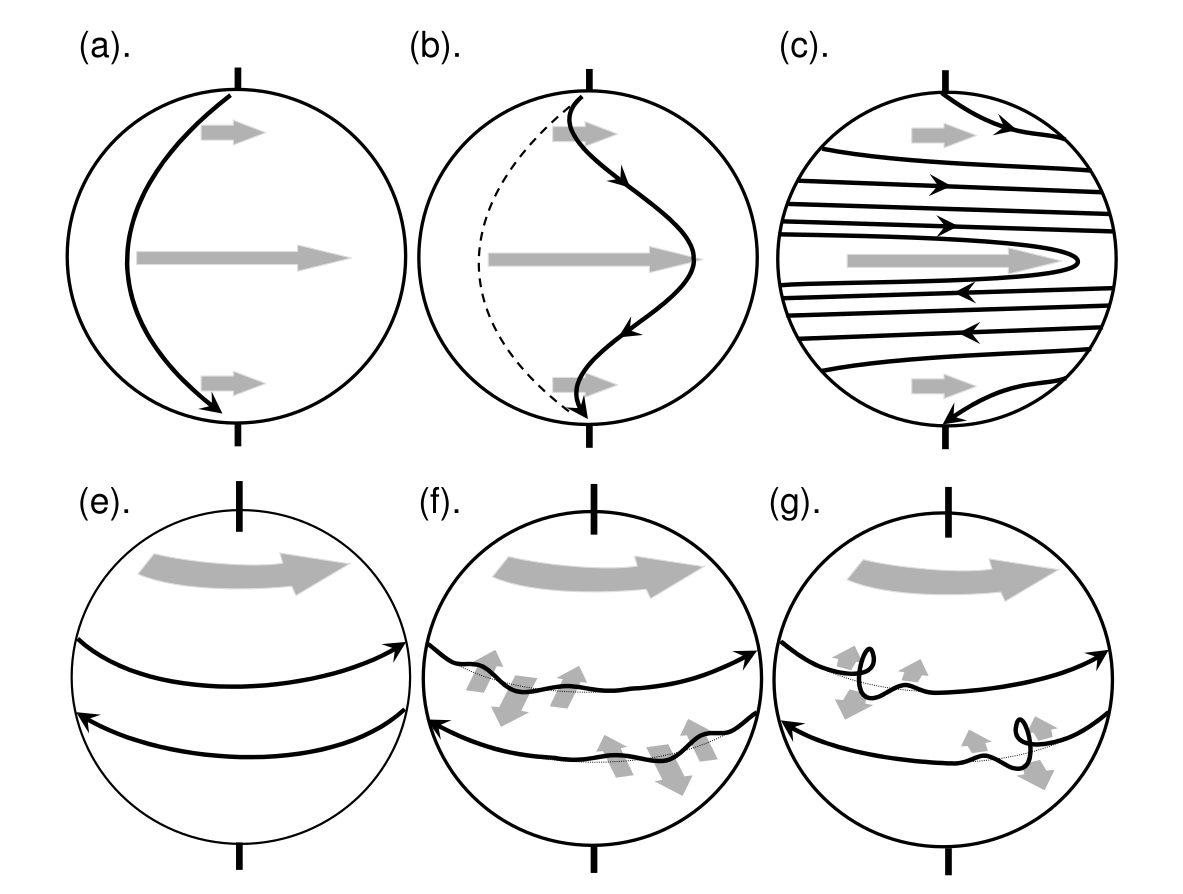
\includegraphics[width=0.7\textwidth]{figuras/babckok_model.png}
%Landi et al. (2016)\\
%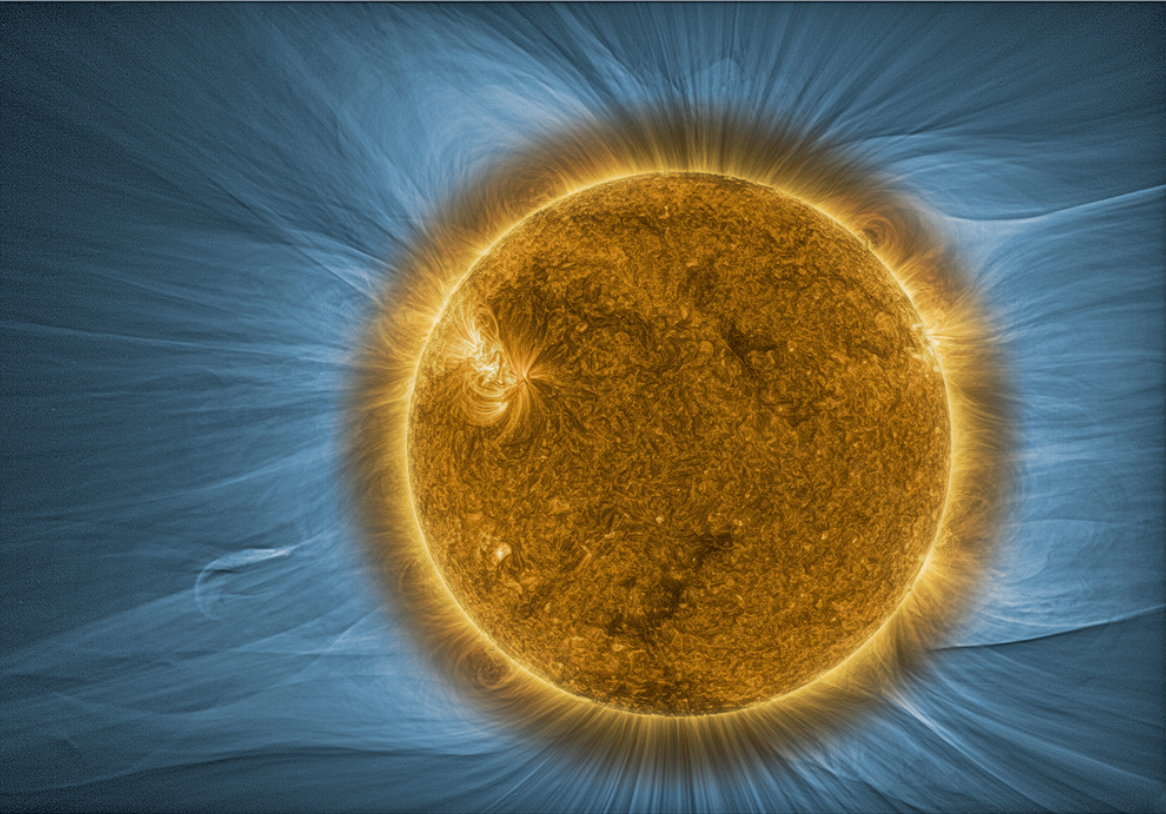
\includegraphics[width=0.6\textwidth,height=0.5\textwidth]{figuras/landi.png}
%\end{center}
%\column{0.5\textwidth}
%\begin{center}
%\bu Solar dynamo $\rightarrow$ B(t).\\
%\vskip 0.5cm
%\bu Mínima: Global dipolo, few SSs/ARs.\\
%\vskip 0.5cm
%\bu Maxima: Multipole, many SSs/ARs.\\
%\vskip 0.5cm
%\bu Period $\sim$ 11 years\\

%\end{columns}


%\vspace{-0.55cm}
%\begin{center}
%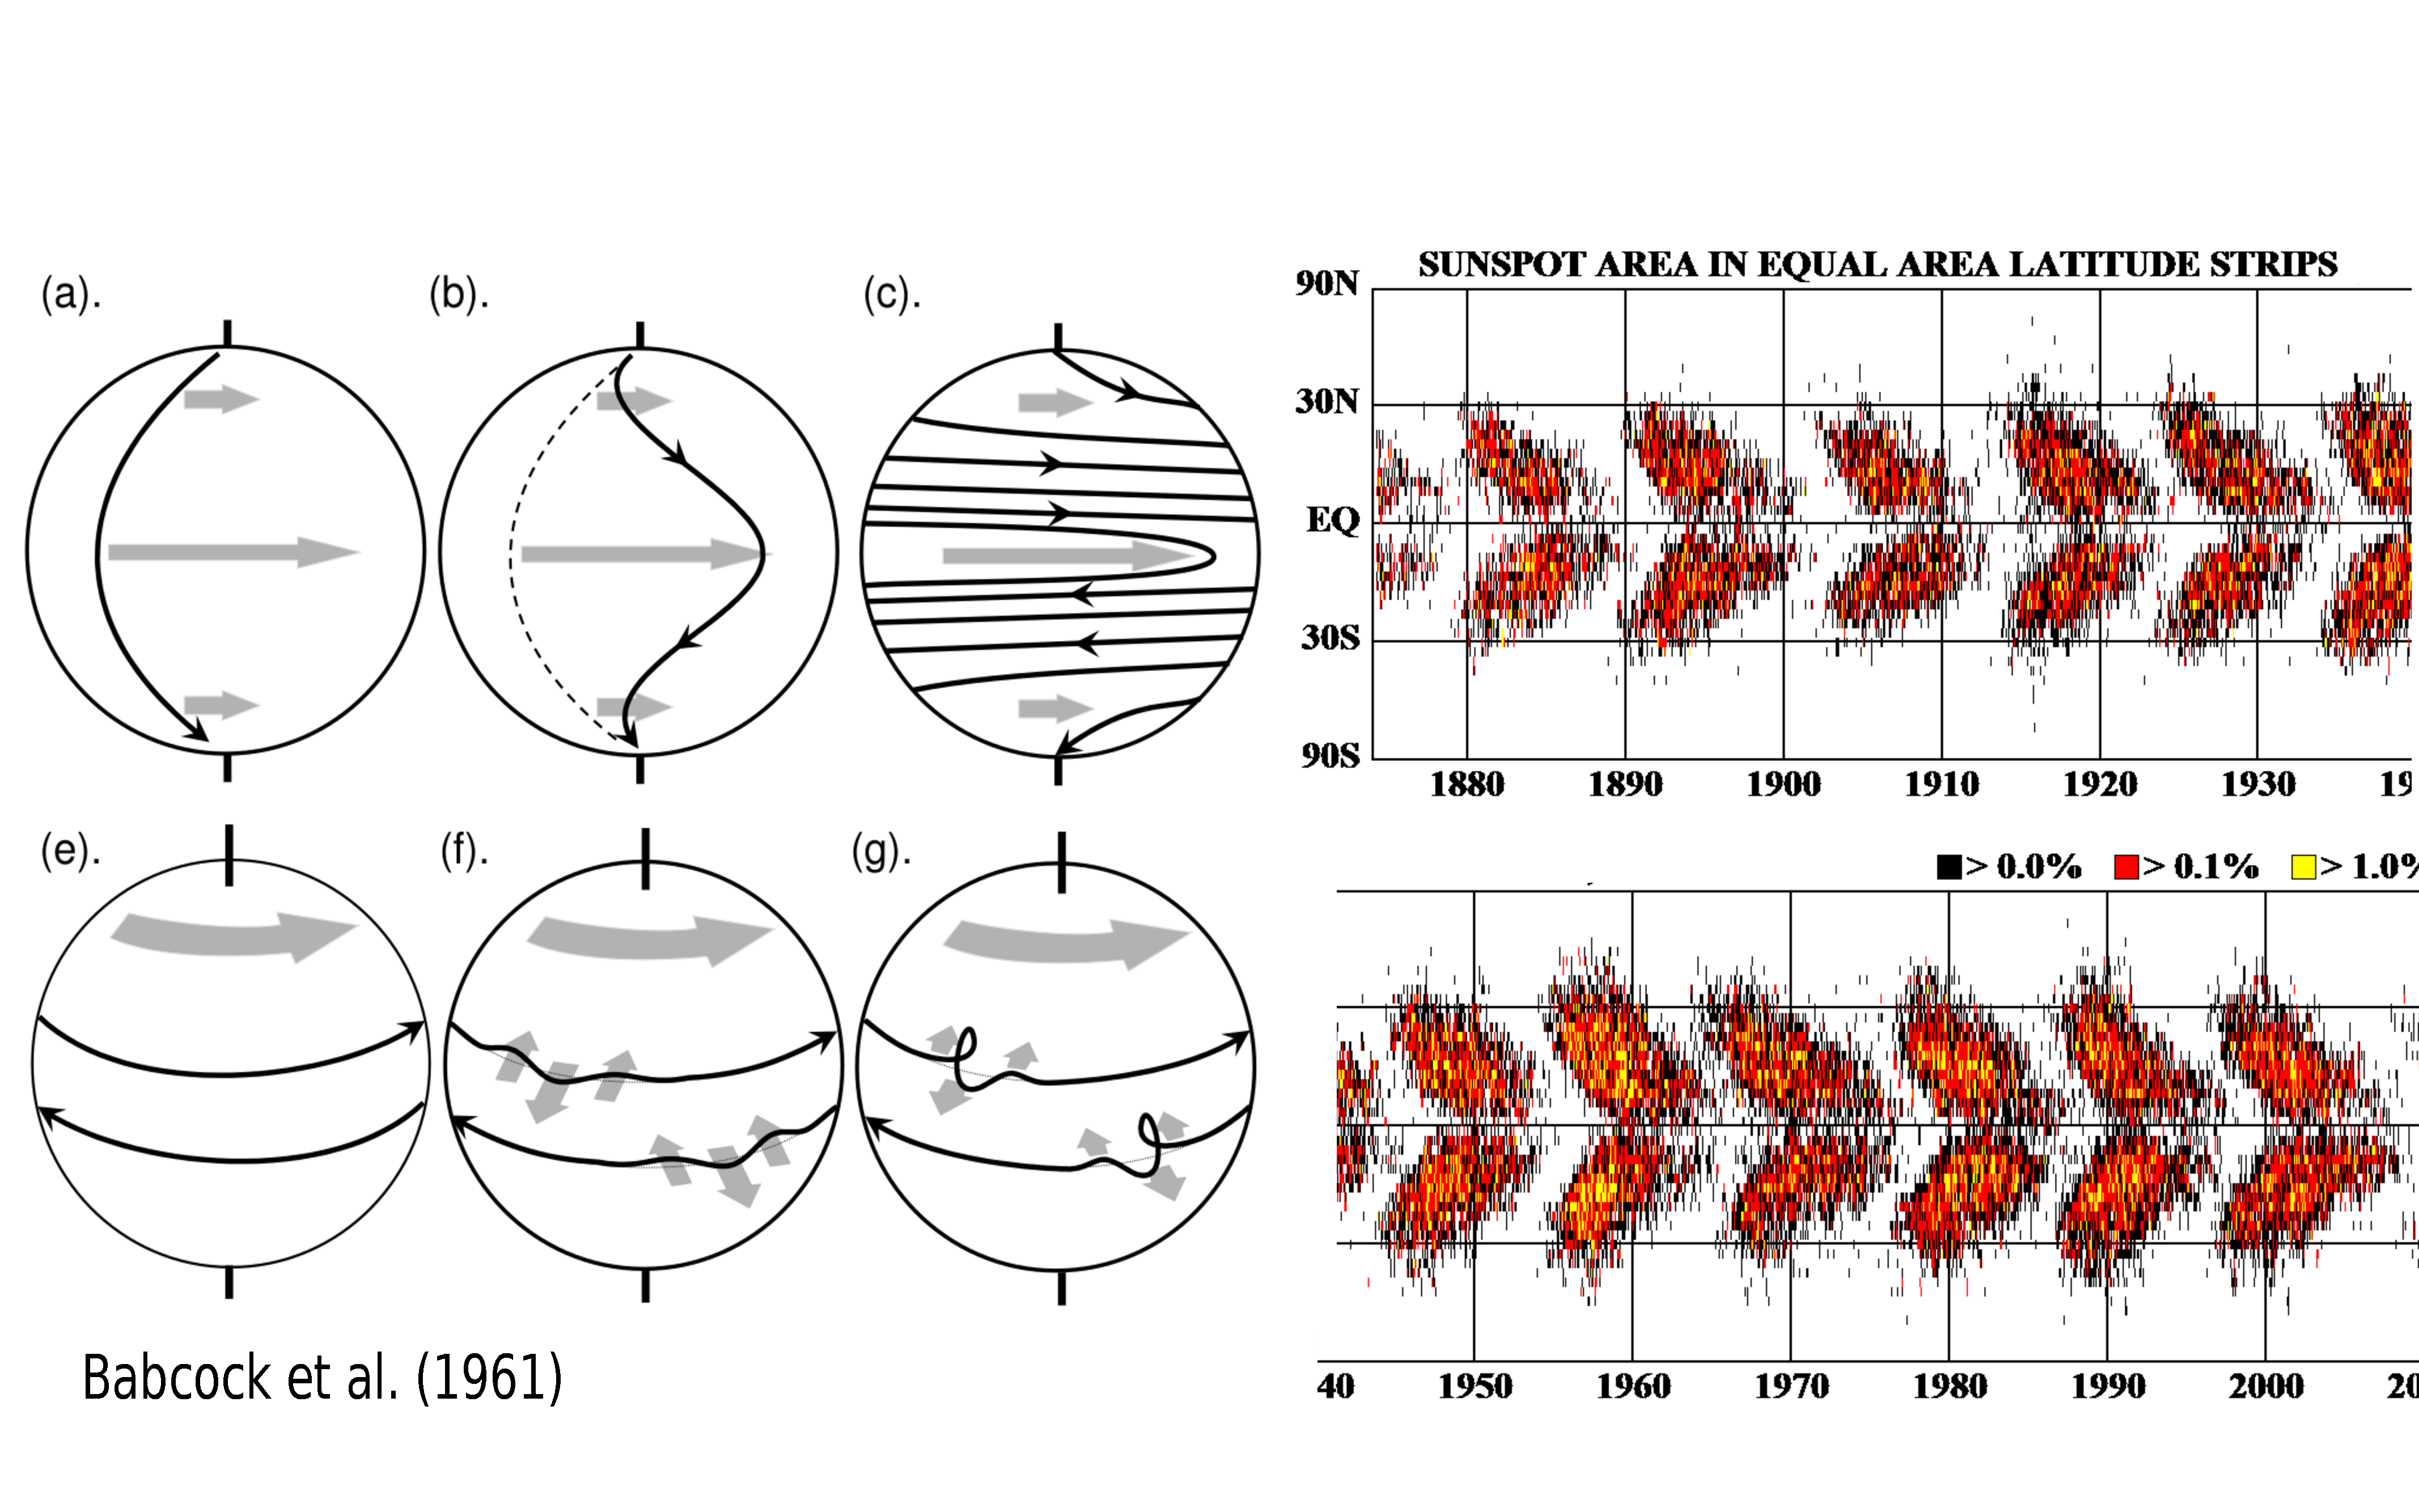
\includegraphics[width=.6\textwidth]{figuras/butterfly-diagram_recorte.pdf}
%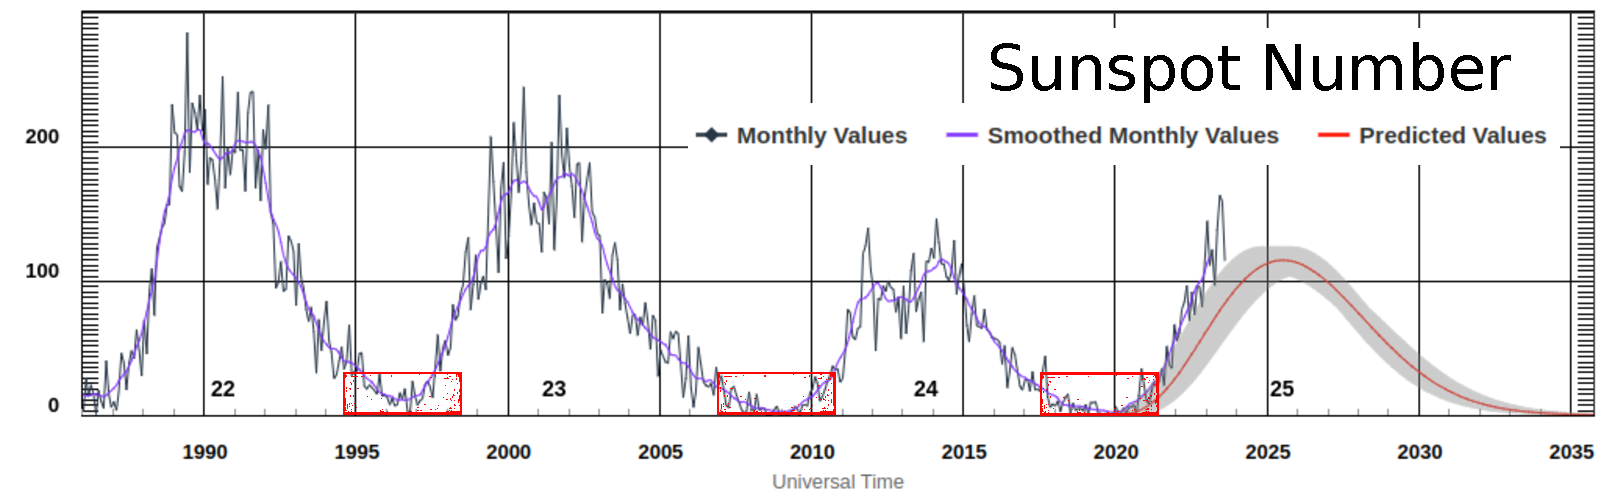
\includegraphics[width=0.99\textwidth]{figuras/conteo_manchas_full.pdf}
%\end{center}
%\vskip -0.5cm
%Space weather prediction center (NOAA)
%}
%}
%----------------------------------------
%{
%\setbeamercolor{title}{fg=blue}
%\setbeamercolor{normal text}{fg=black}
%\setbeamercolor{frametitle}{fg=blue}
%\usebeamercolor[fg]{normal text}
%\usebackgroundtemplate{{\includegraphics[width=\paperwidth]
%{figuras/fondo_poster_70x90cm.pdf}}}
%\frame{
%\titulo{Rotations Selected from each Minima}
%\footnotesize
%\vspace{-0.8cm}
%\begin{columns}
%\column{0.2\textwidth}
%\centering
%\vspace{-4cm}

%\column{0.8\textwidth}
%\begin{center}
%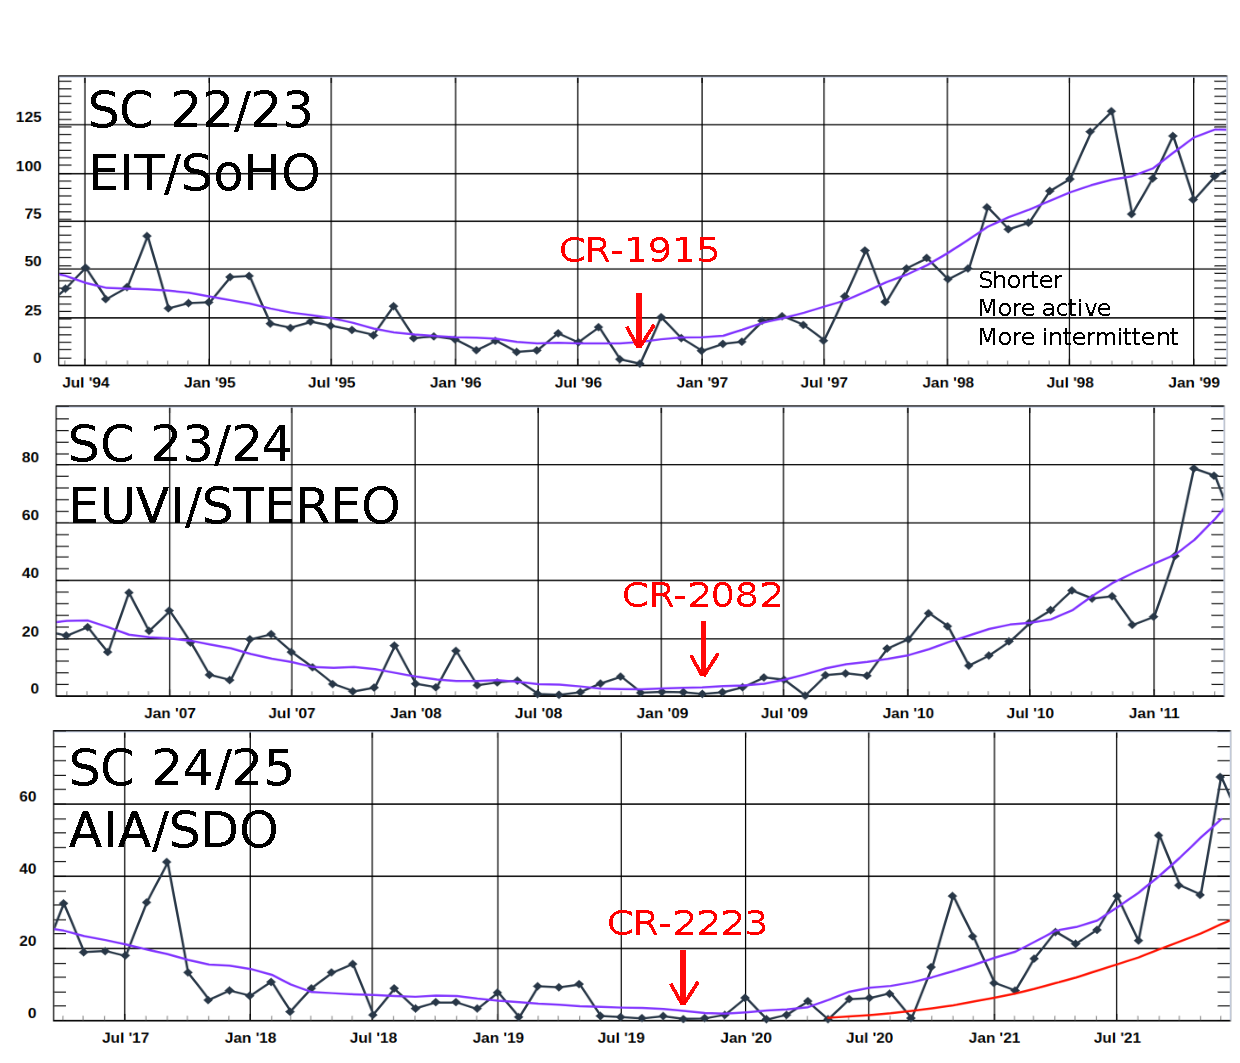
\includegraphics[width=0.99\textwidth,height=0.75\textwidth]{figuras/ciclos_ssn_recorte3_ingles.pdf}
%\end{center}
%\end{columns}
%}
%}

%------------------- tomography
{
\setbeamercolor{title}{fg=blue}
\setbeamercolor{normal text}{fg=black}
\setbeamercolor{frametitle}{fg=blue}
\usebeamercolor[fg]{normal text}
\usebackgroundtemplate{{
\includegraphics[width=\paperwidth]
{figuras/fondo_poster_70x90cm.pdf}}}
\frame{
\titulo{Tomography}
\footnotesize
\vskip 0.1cm
{\bf Unknown:} \rojo{3D distribution of a certain quantity $\bx_i$} (e.g. $\Ne$) for each cell volume $i$ within an object (e.g. the solar corona), under optically thin regime (e.g. WL)\\
\vskip 0.1cm
{\bf Knowns:} 
\begin{itemize} 
\item[\bu] \azul{Intensity vector $\by_j$:} measurement in each \azul{pixel $j$} of each image of a time-series providing different view angles.\\
\item[\bu] \azul{\emph{Proyection} matrix $\bA_{ji}$:} depending on the \azul{geometry} (e.g. solar rotation, telescope orbit) and the involved \azul{physical process} (e.g. Thomson scattering).


\begin{columns}
\column{0.6\textwidth}
\begin{center}
\figu{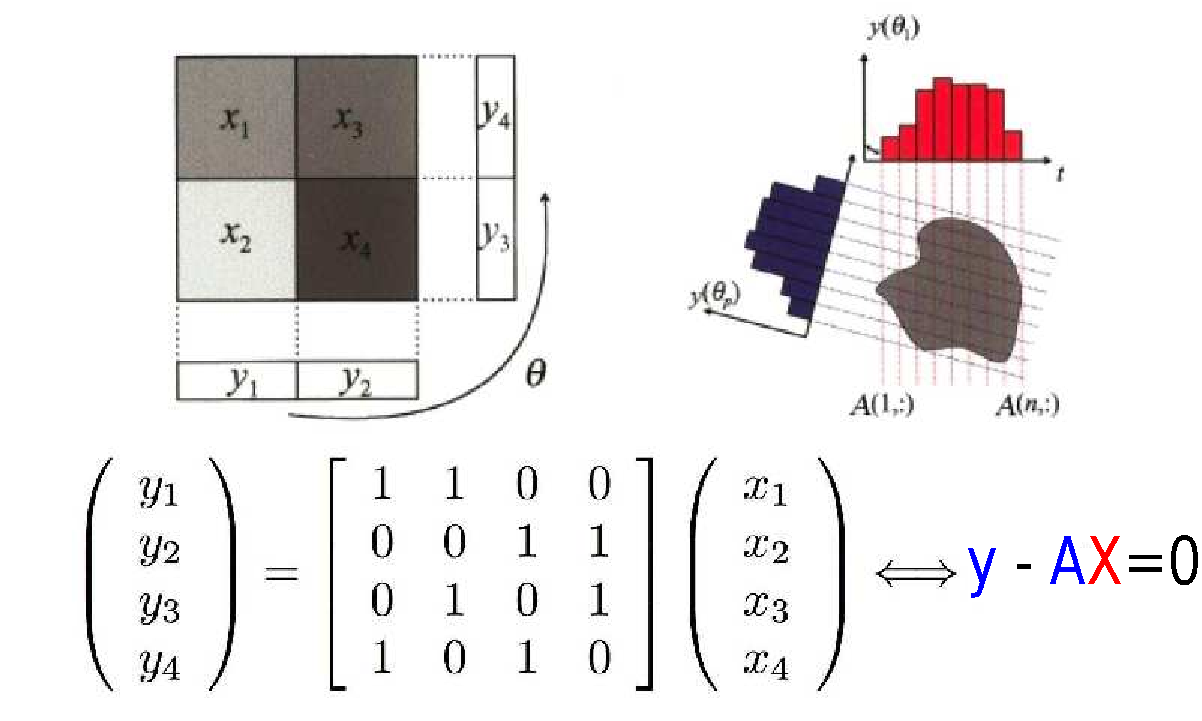
\includegraphics[width=0.7\linewidth]{figuras/tom_sketch_2.pdf}}
\end{center}

\column{0.4\textwidth}
Tomographic reconstruction\\


C2-SRT \red{(N$_e$)} \hfill $2.5 - 6.5 \mrsun$\\

%\scriptsize{\hfill (Altschuler \& Perry, 1972)\\}

%EUV-SRT \red{(N$_e$, T$_e$)} \hfill $1.0 - 1.3 \mrsun$
%\scriptsize{\hfill (Vásquez, Frazin \& Kamalabadi,2009)}
\vskip 0.5cm

EUV-SRT  \\%\red{(N$_e$, T$_e$)} \hfill $1.0 - 1.3 \mrsun$\\
+ LDEM  \red{(N$_e$, T$_e$)} \hfill $1.0 - 1.3 \mrsun$\\
=  \\
DEM Tomography

%\scriptsize{\hfill (Frazin, Vásquez \& Kamalabadi,2009)}
\end{columns}
\item \azul{Solar Rotational Tomography}: it is the solar rotation itself that provides the different viewing angles.

\end{itemize}

}
}

%--------------------------------Coronal radiation
{
\setbeamercolor{title}{fg=blue}
\setbeamercolor{normal text}{fg=black}
\setbeamercolor{frametitle}{fg=blue}
\usebeamercolor[fg]{normal text}
\usebackgroundtemplate{{
\includegraphics[width=\paperwidth]
{figuras/fondo_poster_70x90cm.pdf}}}
\frame{ 
\titulo{Solar Rotational Tomography (SRT)}
\begin{columns}
%\vspace{-1cm}
\column{0.6\textwidth}
\footnotesize
Radiation from the corona is caused by different phenomena
\begin{itemize}
\item K-Corona: Thomson scattering of pothosphere WL $\rightarrow$ diagnostics of $N_e$
\item WL-SRT $\rightarrow$ 3D $N_e$
\item Altschuler \& Perry (1972)
\end{itemize}
%\salto
\salto

%EUV images of a complete solar cycle. Images taken in the ${\rm 195 \AA}$ band of the EIT/SoHO instrument.
\begin{itemize}
%item The maximum phase shows a large number of ARs and these appear in two well-defined latitude bands.
\item E-Corona: Electronic decay of Iron ions emitting in EUV $\rightarrow$ diagnostics of $N_e$ and $T_e$
\item EUV-SRT $\rightarrow$ 3D EUV emissivity $\rightarrow$ 3D DEM $\rightarrow$ 3D $N_e$ and $T_e$
\item Frazin et al. (2009), Vasquez et al. (2009)
%The minimum phase shows a marked decrease in ARs, characterizing the quiescent corona.
\end{itemize}

\column{0.4\textwidth}
\begin{center}
\azul{White light Coronagraph}
%\movie[externalviewer]{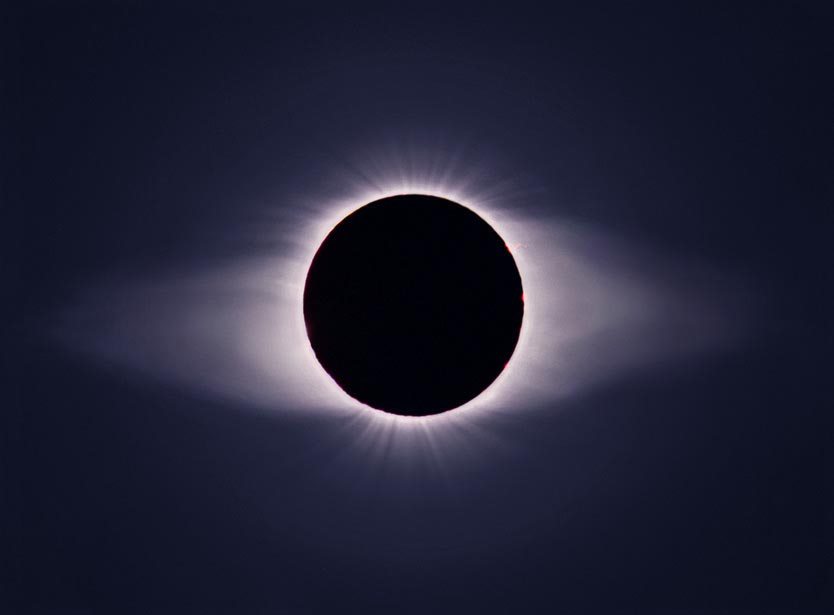
\includegraphics[width=0.45\textheight, keepaspectratio]{figuras/streamer_minimo_solar.jpg}}{lasco_2019.mp4}
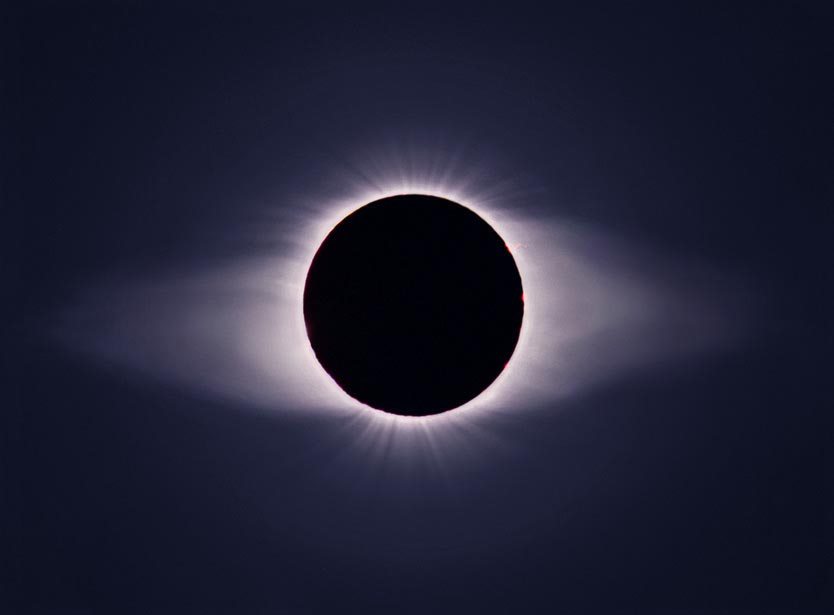
\includegraphics[width=0.9\textwidth]{figuras/streamer_minimo_solar.jpg}
\mediosalto
%\azul{Ciclo en EUV}
%\framebox{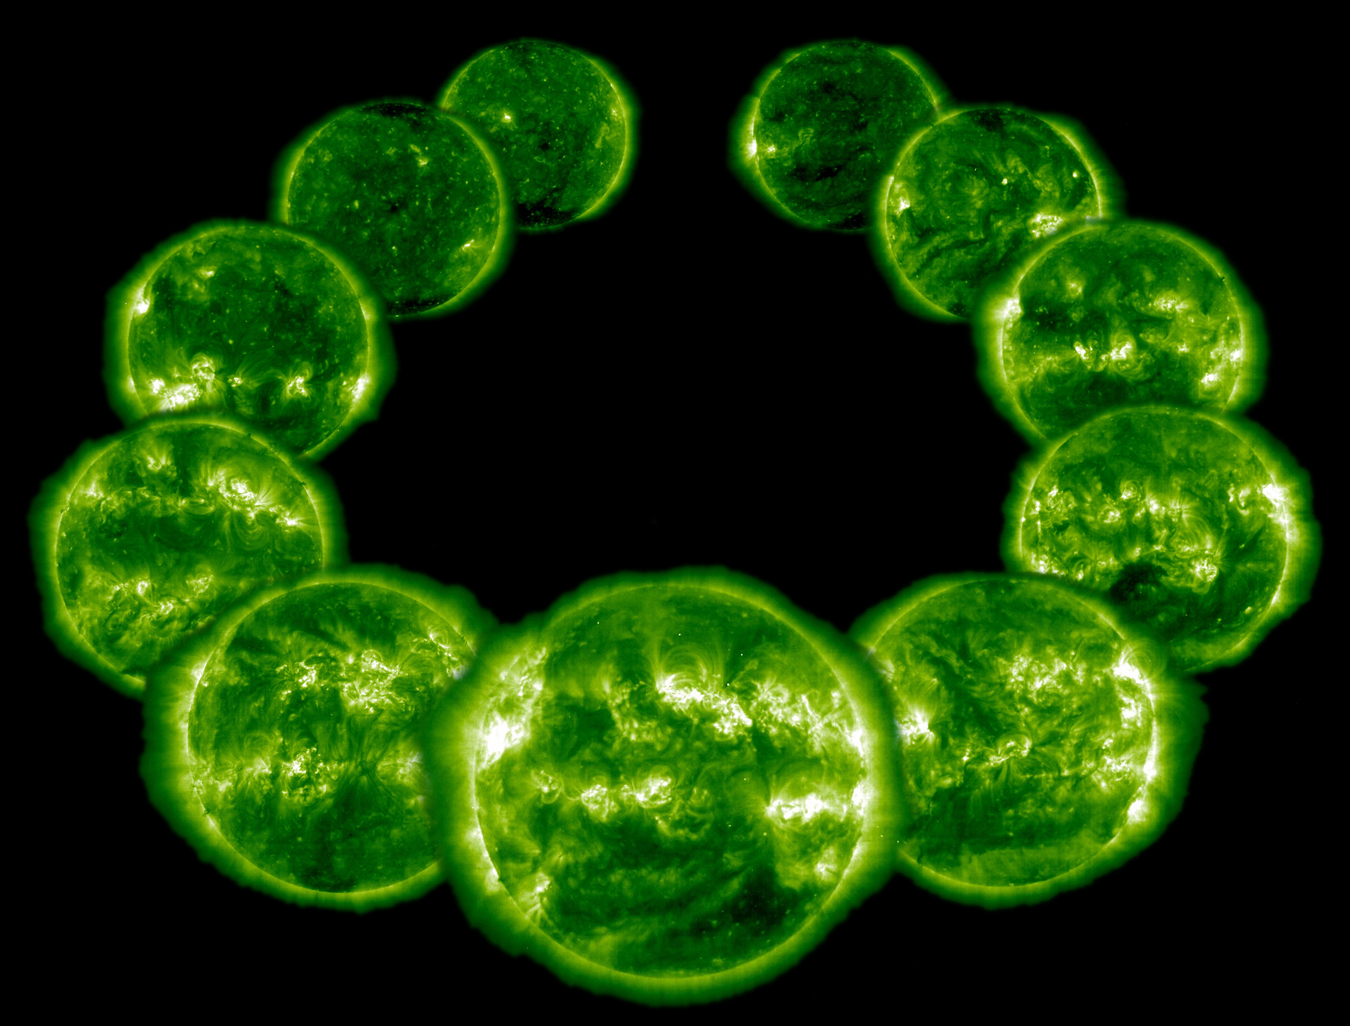
\includegraphics[width=0.9\textwidth]{figuras/ciclo_solar.jpg}}
\end{center}
\azul{EUV Telescope}
\centering
%\movie[externalviewer]{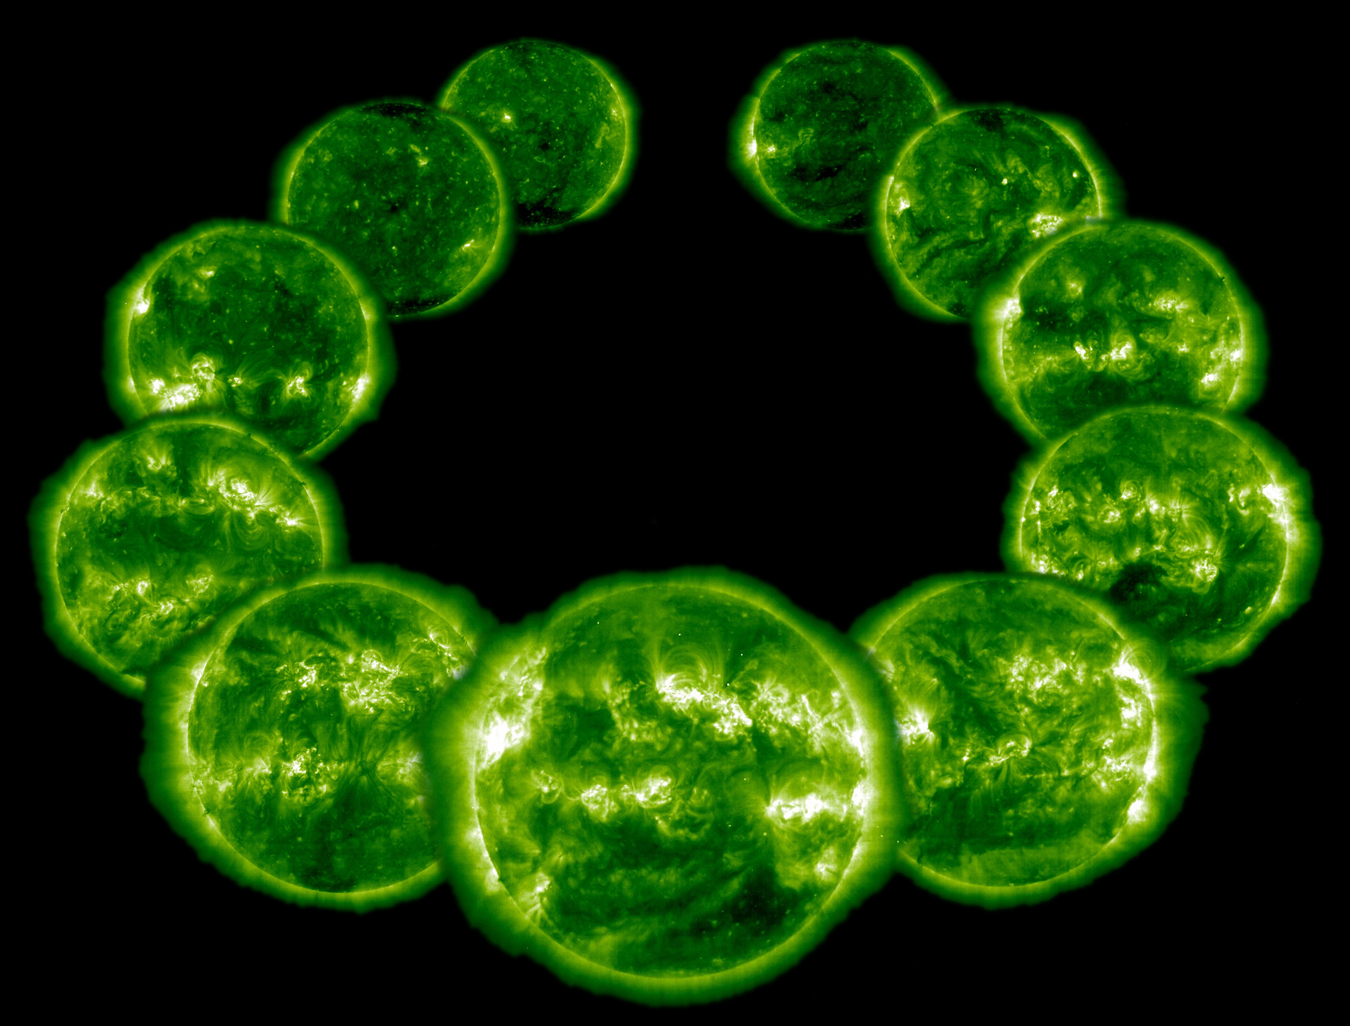
\includegraphics[width=0.45\textheight, keepaspectratio]{figuras/ciclo_solar.jpg}}{2019_AIA_193.mp4}
%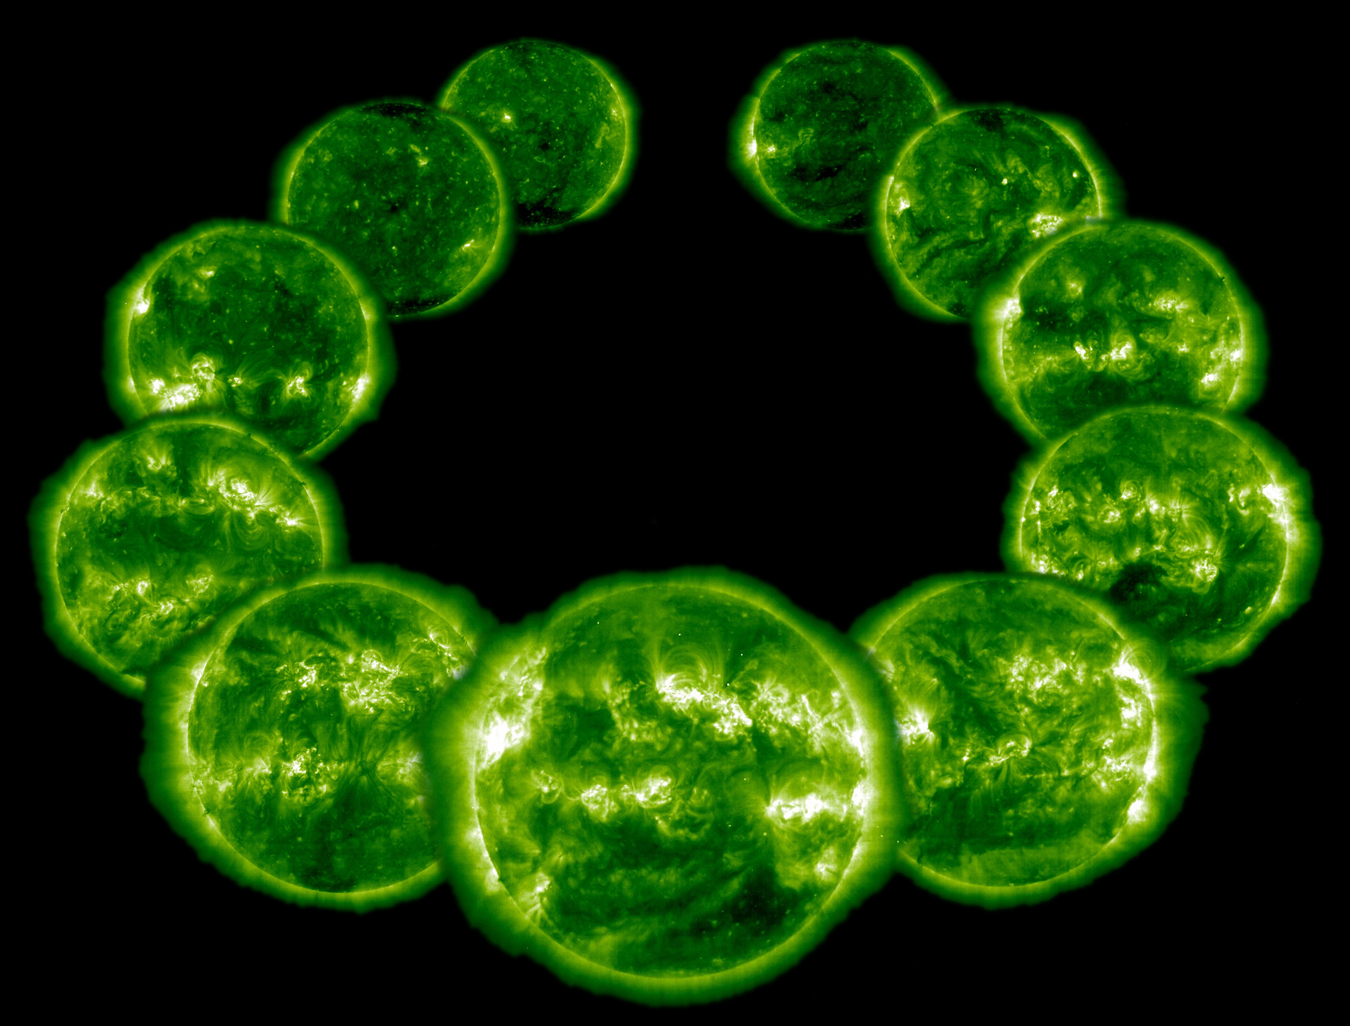
\includegraphics[width=0.9\textwidth]{figuras/ciclo_solar.jpg}
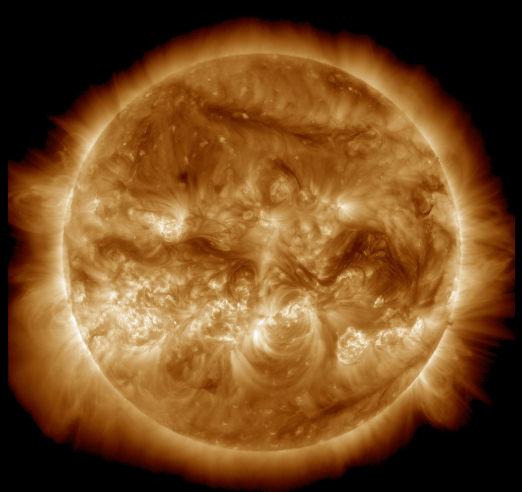
\includegraphics[width=0.7\textwidth]{figuras/aia_charla.png}
\end{columns}
}
}
%------------------------------
%\begin{frame}
%\titulo{¿Que es la Tomografía Solar?}
%\footnotesize
%\vskip 0.1cm
%\rojo{\bf Unknown:} \rojo{3D distribution of a certain quantity $bx_i$} (e.g. $N_e$) for each cell volume $i$ within an object (e.g. the solar corona), under optically thin regime (e.g. coronal white light)\\
%\rojo{\bf Incógnita:} \rojo{Distribución en 3D de una determinada cantidad $\bx_i$} (por ejemplo, $N_e$) para cada volumen de celda $i$ dentro de un objeto (p. ej., la corona solar), en régimen óptico delgado (p. ej., luz blanca coronal)

%\vskip 0.1cm
%\azul{\bf Dato:} 
%\begin{itemize} 
%\item \azul{Intensity vector $by_j$:} measurement in each \azul{pixel $j$} of each image of a time-series providing different view angles.\\
%\item \azul{Vector de intensidad $\by_j$:} medición en cada \azul{pixel $j$} de cada imagen de una serie temporal proporcionando diferentes ángulos de visión.\\

%\item \azul{\emph{Proyection} matrix $bA_{ji}$:} depending on the \azul{geometry} (e.g. solar rotation, telescope orbit) and the involved \azul{physical process} (e.g. Thomson scatt.).

%\item \azul{Matriz de proyección $\bA_{ji}$:} depende de la \azul{geometría} (p. ej., rotación solar, órbita del telescopio) y el %\azul{proceso físico} involucrado (p. ej., Thomson scatt.).

%\begin{columns}
%\column{0.6\textwidth}

%\begin{center}
%{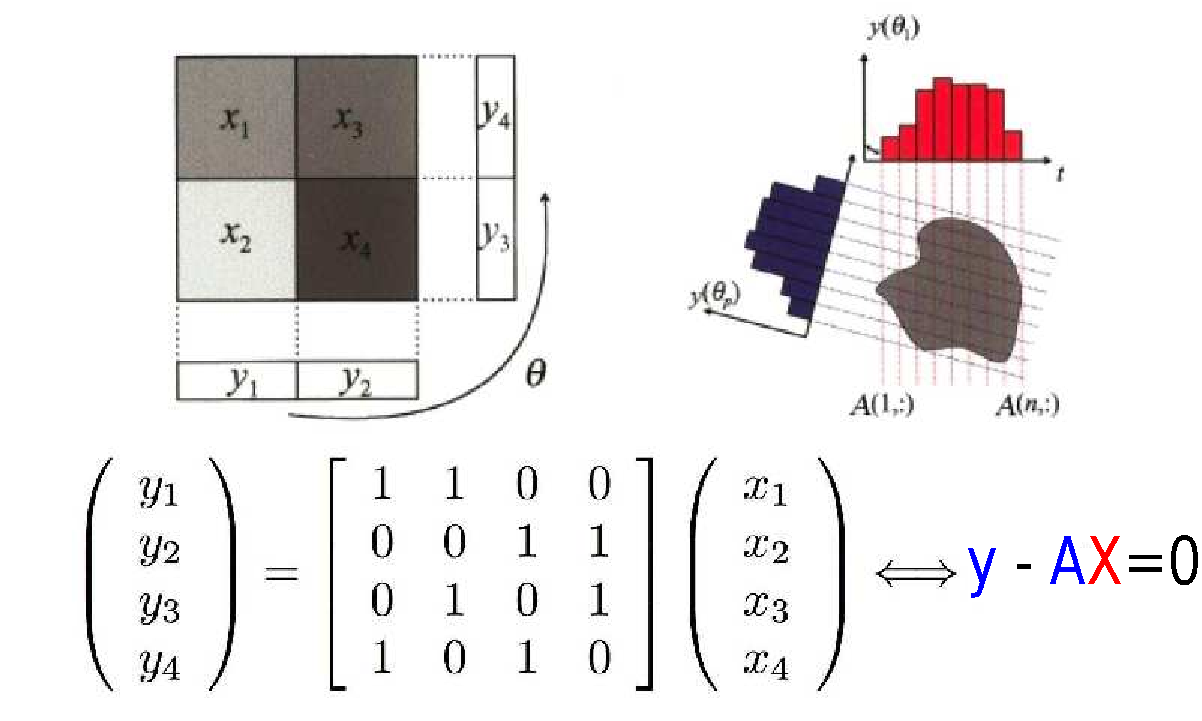
\includegraphics[width=0.9\linewidth]{figuras/tom_sketch_2.pdf}}
%\end{center}

%\column{0.4\textwidth}
%Reconstrucción tomográfica\\


%C2-SRT \red{(N$_e$)} \hfill $2.5 - 6.5 \mrsun$\\
%\scriptsize{\hfill (Altschuler \& Perry, 1972)\\}

%EUV-SRT \red{(N$_e$, T$_e$)} \hfill $1.0 - 1.3 \mrsun$
%\scriptsize{\hfill (Vásquez, Frazin \& Kamalabadi,2009)}

%\scriptsize{\hfill (Frazin, Vásquez \& Kamalabadi,2009)}
%\end{columns}
%\item \azul{Tomografía rotacional solar}: la rotación solar proporciona los ángulos de visión necesarios.
%\item \azul{$bA$} is a very large sparse matrix, 
% \emph{global optimization} of \emph{objective function}:
%$$
%f(\rojo{{\bf x}}) \ \ =  \ \  
%\| \azul{\by} - \azul{\bA\,\cdotp\,} \rojo{{\bf x}} \|^2 \ \ + \ \
%{\sf regularization\ terms}
%$$
%\end{itemize}
%\end{frame}









%---------------------------------EXTRA SRT
\begin{frame}%[noframenumbering]
\titulo{The SRT Problem}
\footnotesize
\begin{center}
The signal recorded by the $j$-th pixel is given by:
\vskip 0.1cm
\figu{
$\azul{I_j} \ = \ \azul{ \int_{\textsf{LOS}_j} \ \textsf{d}l} \  
\azul{w(l)} \ \rojo{x(\azul{l})} 
\ \ \rightarrow \ \
\azul{\boldsymbol{I}} = \azul{\boldsymbol{A}\,\cdotp\,} \rojo{{\boldsymbol{X}}} $
}
\end{center}
\hskip 1.45cm
\azul{\ $\mathbf{I}$}: Vector of $\azul{J}$ elements $\azul{I_{j}}$, all pixels in all images.\\
\hskip 1.5cm
\azul{\,$\mathbf{A}$}: Large sparse matrix of $\azul{J\times I}$ elements $\azul{a_{j,i}}$, purelly geometrical.\\
\hskip 1.5cm
\rojo{\,$\rojo{\mathbf{X}}$}: Vector of $\azul{I}$ elements $\rojo{x_{i}}$, the discrete 3D distribution of the unknown:\\
\begin{center}
\begin{columns}
\column{0.5\textwidth}
\centerline{\bf \underline{WL-SRT}}
\vspace{-.5cm}
\begin{eqnarray*}
\rojo{x \left(\azul{{\bf r}}\right)} &=& 
\rojo{\Ne\left(\azul{{\bf r}}\right)}\\
\azul{w({\bf r})} &=& \azul{S_{\textsf{Thomson}}({\bf r})}
\end{eqnarray*}
\ \\
\column{0.5\textwidth}
\centerline{\bf \underline{EUV-SRT}}
\vspace{-.5cm}
\begin{eqnarray*}
\rojo{x \left(\azul{{\bf r}}\right)} &=&
\rojo{FBE_k\left(\azul{{\bf r}}\right)} \equiv \int_{0}^{\infty} \mathrm{d} \lambda \ \phi_k(\lambda)\ \eta (\mathbf{r}, \lambda)
\\
\azul{w({\bf r})} &=& \azul{1}
\end{eqnarray*}
\end{columns} 
\vskip 0.5cm
Solution: global optimization problem with cost function (of dimension-$I$):
\vskip 0.1cm
\figu{
$
f(\rojo{\boldsymbol{X}})
\ = \ 
\| \azul{\boldsymbol{I}} - \azul{\boldsymbol{A}}\cdotp\rojo{\boldsymbol{X}} \|^2
\ + \ 
p\ \|  \azul{\bR}\cdotp\rojo{\boldsymbol{X}}   \|^2
$
}
\\
\underline{1st term:} Difference between data and synthetic images.\\
\underline{2nd term:} Regularization of the solution.
\end{center}
\end{frame}

%--------------------------C2-SRT
{
\setbeamercolor{title}{fg=blue}
\setbeamercolor{normal text}{fg=black}
\setbeamercolor{frametitle}{fg=blue}
\usebeamercolor[fg]{normal text}
\usebackgroundtemplate{{
\includegraphics[width=\paperwidth]
{figuras/fondo_poster_70x90cm.pdf}}}
\frame{
\titulo{WL-SRT Validation of AWSoM}
\begin{center}
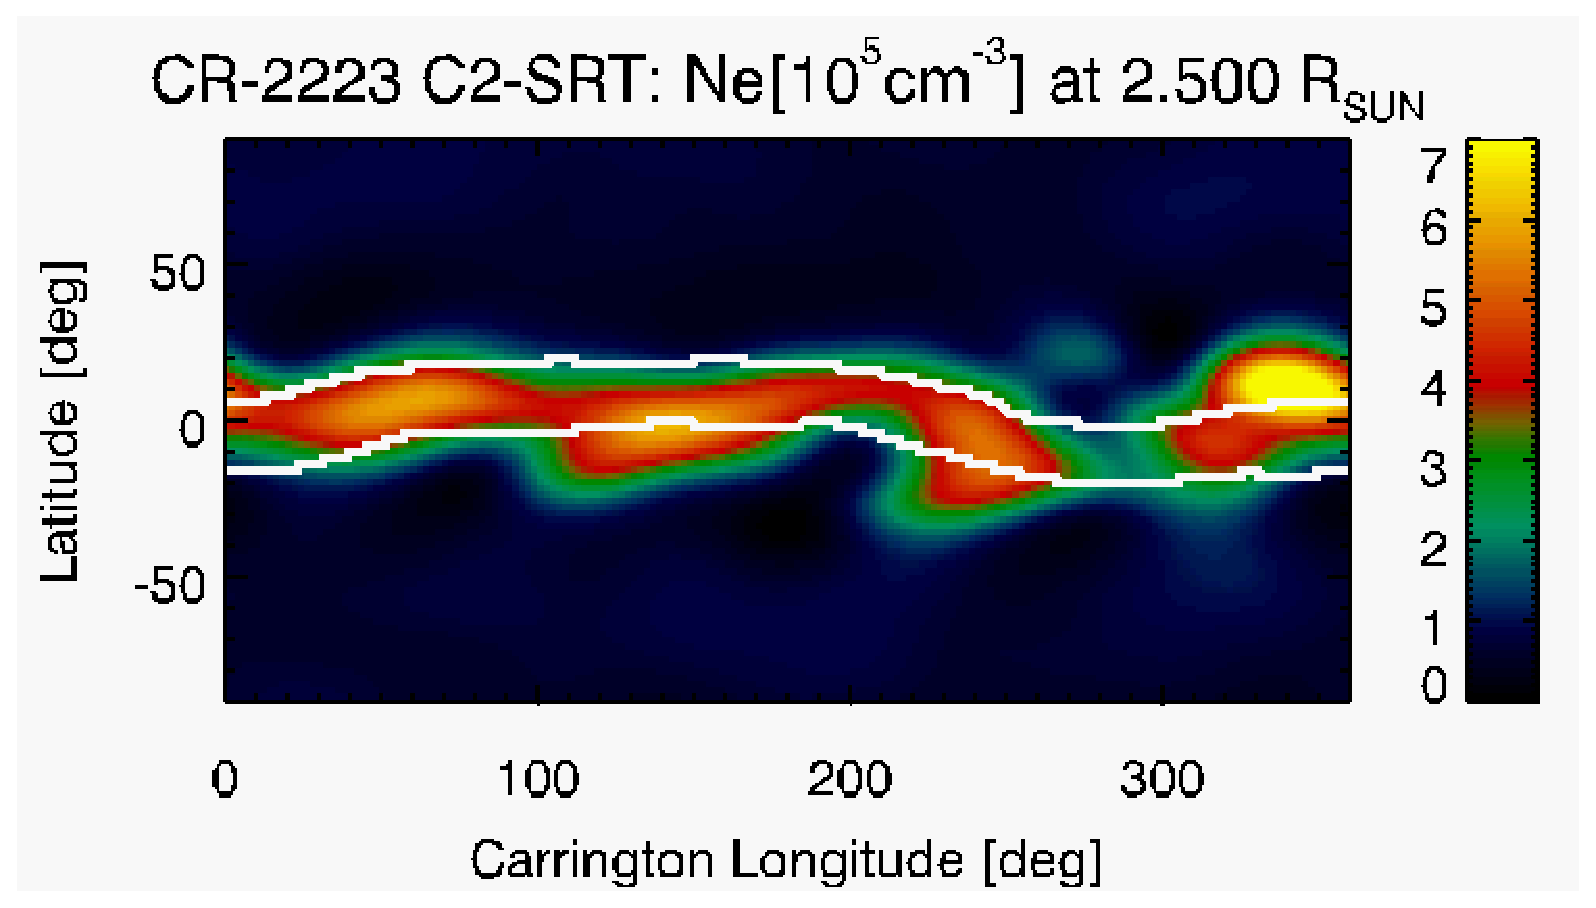
\includegraphics[width=0.43\textwidth,clip=]{figuras/map_LASCOC2pB_CR2223_24hr-Cadence_Rmin225_Rmax825_IRmin25_IRmax60_60x60x120_BF2_r3D_l25e-5_vfinal_interpolado_2500_Rsun2223.eps}
%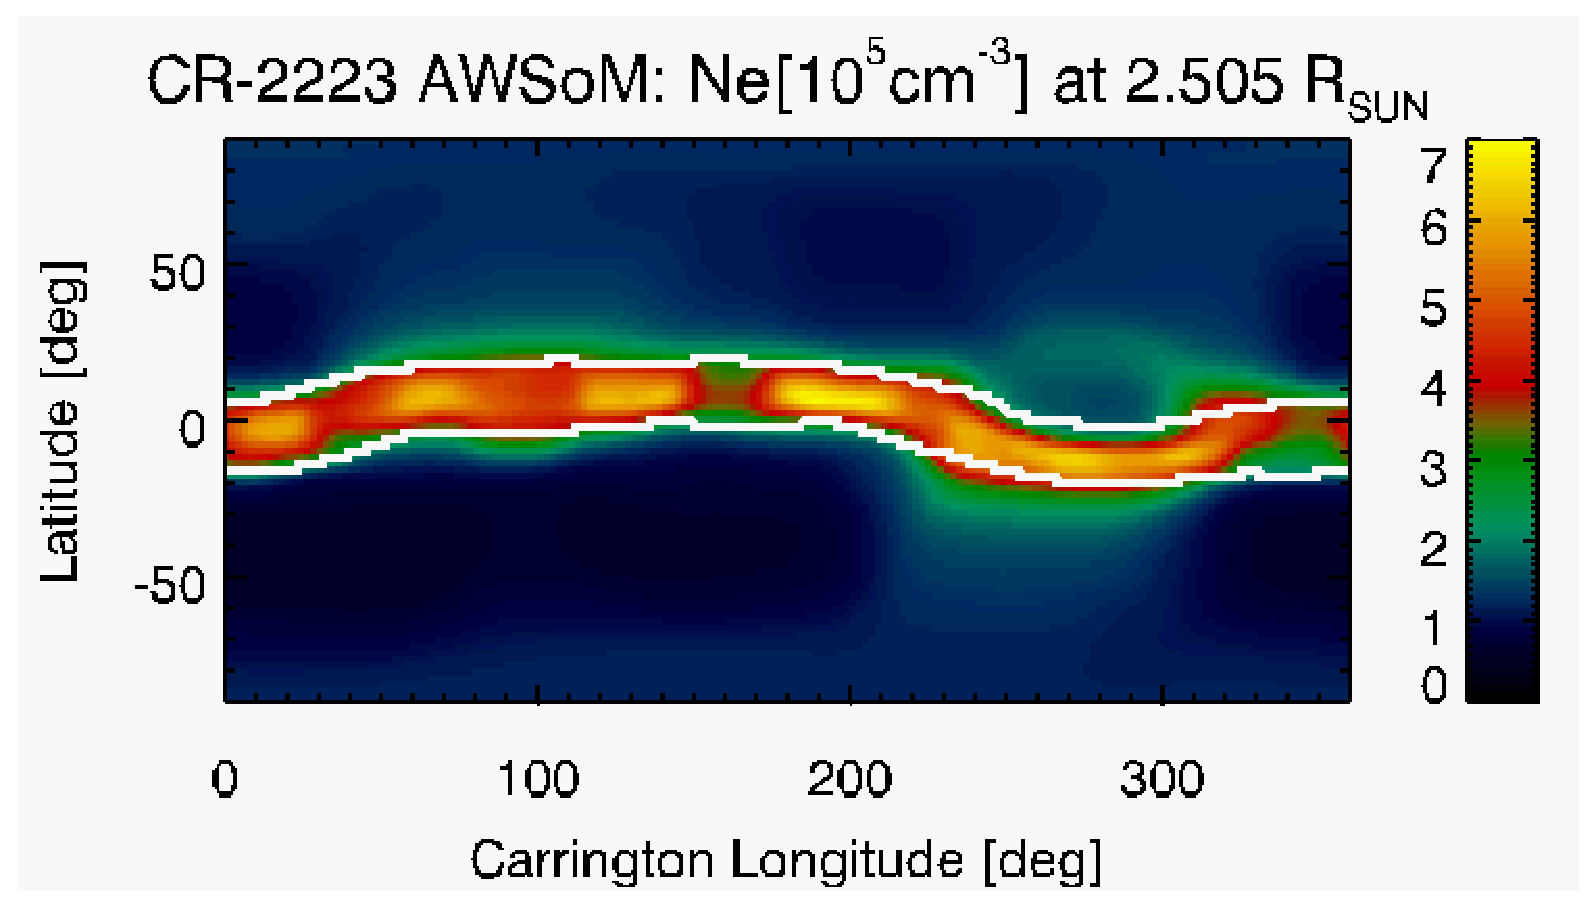
\includegraphics[width=0.33\textwidth,clip=]{figuras/map_Ne_awsom_2223_ener_new_2505_Rsun2219.eps}
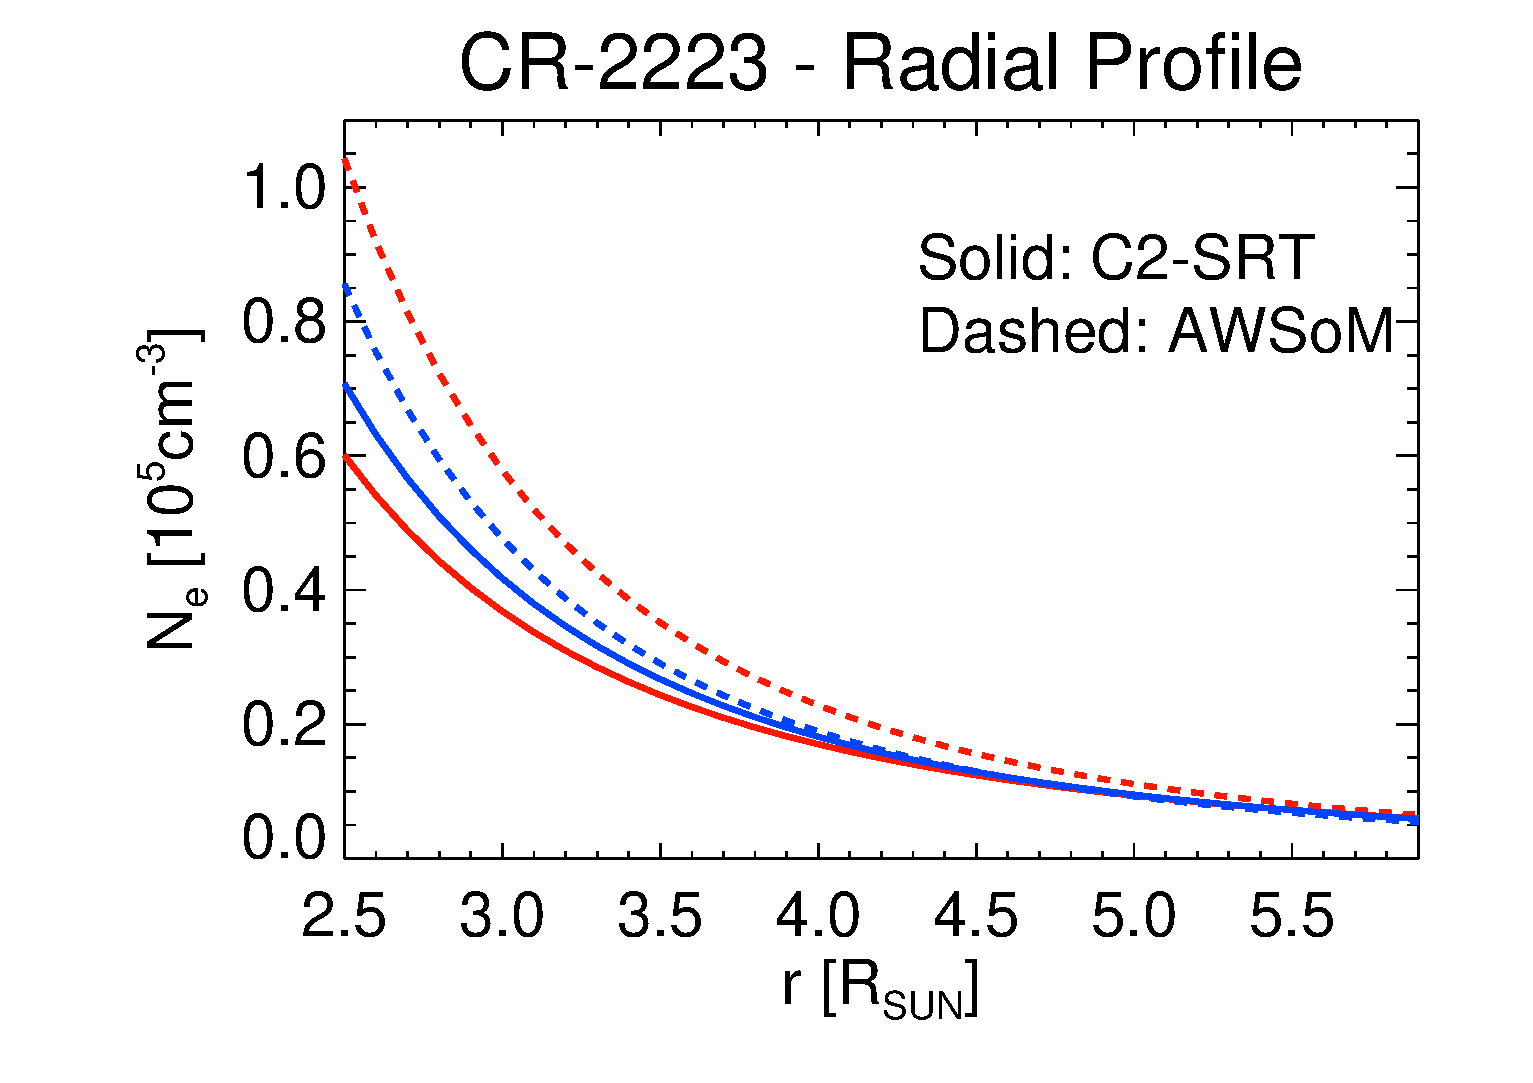
\includegraphics[width=5.4cm,height=3.3cm,clip=]{figuras/perfil_paper_necr2223_alto_simplepot.eps}
\end{center}

%\scriptsize
%\bu Good overall consistency in shape and size of streamer y CHs.
%$$N_e^{\rm (C2-SRT)}(r) = N_0\,\left(\,r/2.5\,\mrsun\right)^{-p} \rightarrow \langle \l \rangle = \frac{\langle r\rangle}{p} $$ 

\vskip 0.2cm
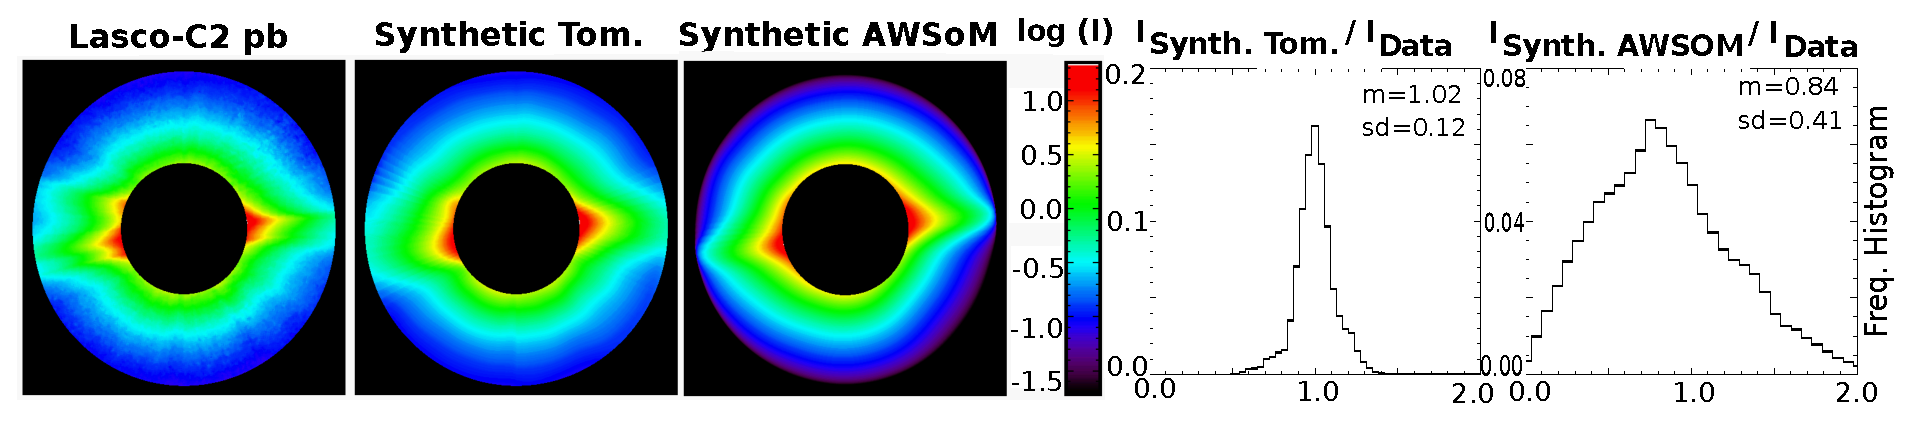
\includegraphics[width=0.99\textwidth,clip=]{figuras/Figura_7_paper_imag_sintetica_2.eps}

%$I_{Synt} \sim \int_{LDV} \mathrm{d}l \, N_e$
%\bu Ne$(r=2.5\,\mrsun) \approx 0.6-0.7\times 10^5\,{\rm cm}^{-3}$ \hfill $I_{Synt} \sim \int_{LoS} \mathrm{d}l \, N_e$ \\

%\bu $\lambda_N\approx 1.4-1.6 \,\mrsun \rightarrow \left<p\right> \approx 2.8-3.3$ (consistent with other studies)\\

%\bu AWSoM overestimates basal density by up to $+75\%$ $\rightarrow$ model's acceleration rates are too low.\\

%\bu AWSoM sobrestima densidad basal en hasta 75\%\\
%\, \, \, \, \, \, \, $\rightarrow$ aceleración del viento es gradual y extendida
\hfill (Lloveras et al. 2022)
}
}

%-------------------> FBE + mamuschkas

\begin{frame}%[noframenumbering]

\vspace{-0.35cm}
\begin{columns}
\noindent
\column{0.075\textwidth}
\vskip 0.8cm
{\footnotesize
\ 171 \AA
\vskip 1.75cm
\ 195 \AA
\vskip 1.65cm
\ 284 \AA
}
\column{\textwidth}
\begin{center}
{\footnotesize
\ \ Data Image \hfill $\rightarrow$ \hfill 3D FBE \hfill $\rightarrow$ \hfill Synthetic Image\ \ \ \
}\\
\framebox{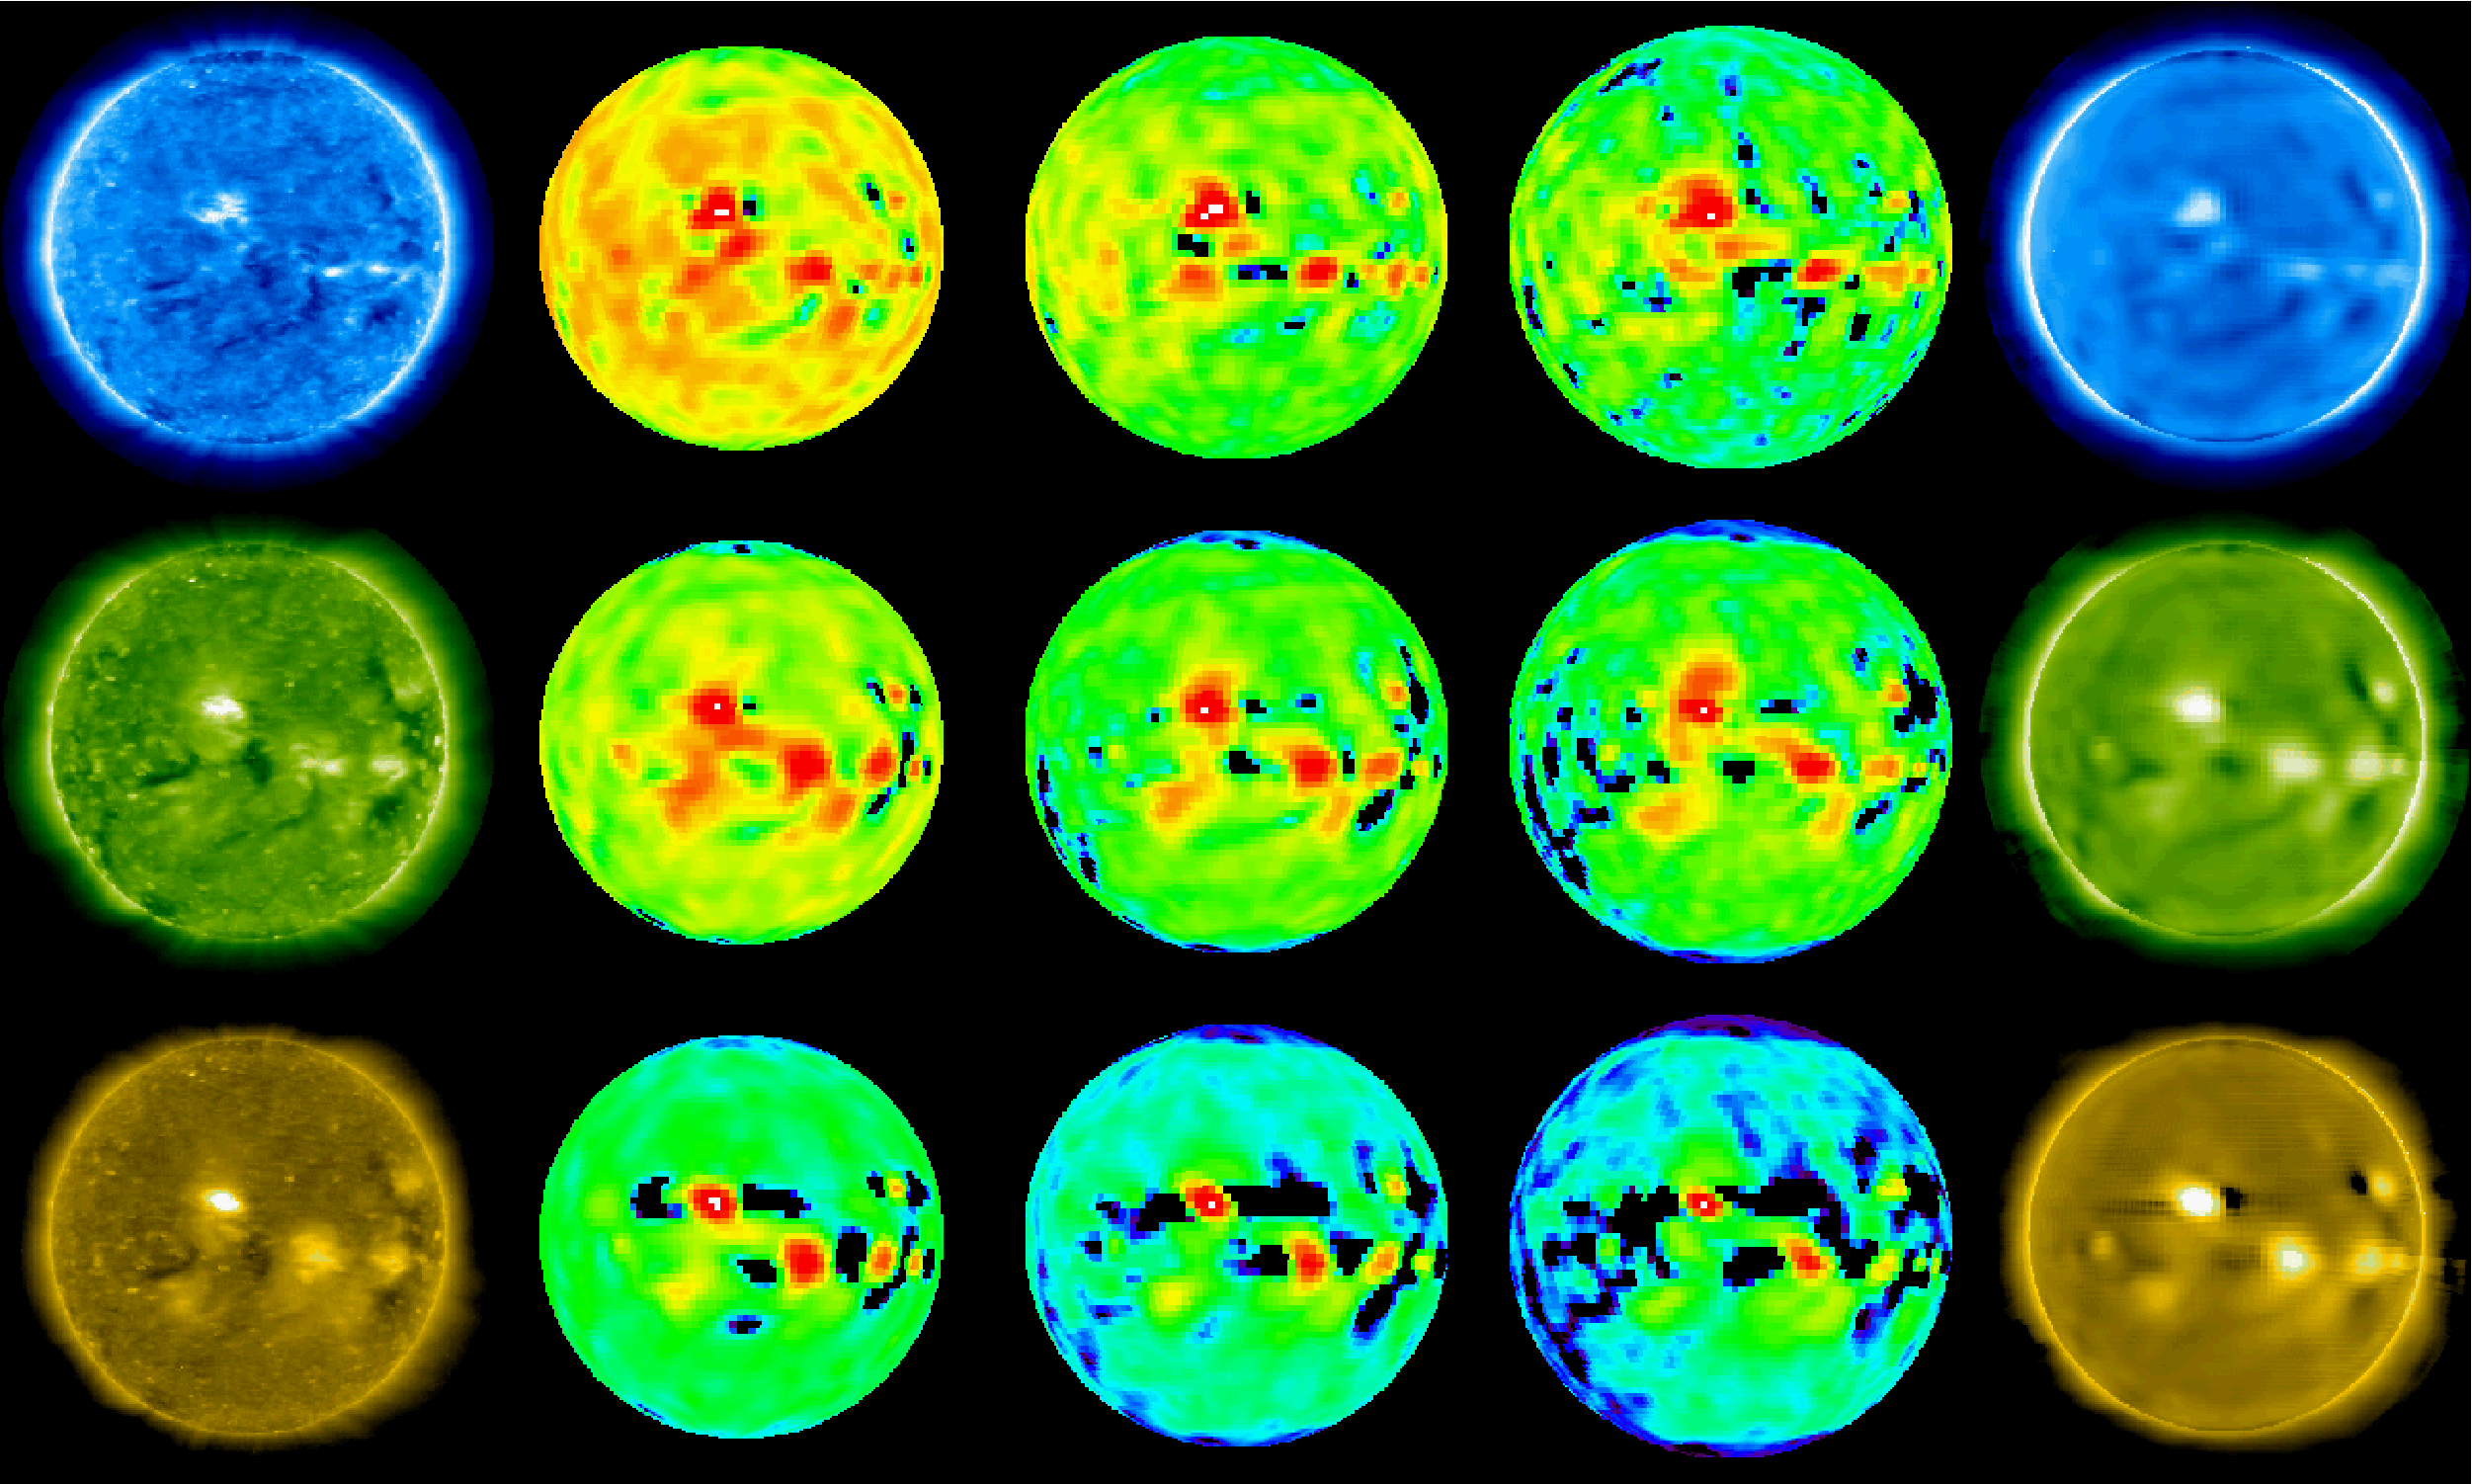
\includegraphics[width=0.95\linewidth]{figuras/frame_050_test.pdf}}\\
\footnotesize
 1.035 $\mrsun$ \hskip 1cm 1.085 $\mrsun$ \hskip 1cm 1.135 $\mrsun$ \hfil
\end{center}
\end{columns}
\begin{columns}
 \column{0.4\textwidth}
 Vásquez et al. (2009)
 \column{0.6\textwidth}
\end{columns}
\end{frame}

%----------------------------------------------

\frame{ 
\titulo{Temperature Response of EUV Bands}
\vspace{-.5cm}
\footnotesize
Space telescopes have EUV detectors, whose filters mainly select Fe lines (T$_e \sim 0.5  - 2.5$ \ MK). \\
%\begin{comment}
%\begin{columns}
% \column{0.5\textwidth}
% Telescopios utilizados:
%\begin{itemize}
% \item Extreme ultraviolet Imaging Telescope (EIT), a bordo de la misión Solar and Heliospheric Observatory (SoHO). Observaciones 1996 - 2006.
% \item Extreme UltraViolet Imager (EUVI), a bordo de las dos naves de la misión Solar TErrestrial Relations Observatory (STEREO). Observaciones 2007 - actualidad. 
% \item Atmospheric imaging Assembly (AIA), a bordo de la misión Solar Solar Dynamic Observatory (SDO). Observaciones 2010 - actualidad. 
%\end{itemize}
%\column{0.5\textwidth}
%\framebox{\includegraphics[width=0.9\textwidth]{figuras/passband_EIT-EUVI.pdf}}
%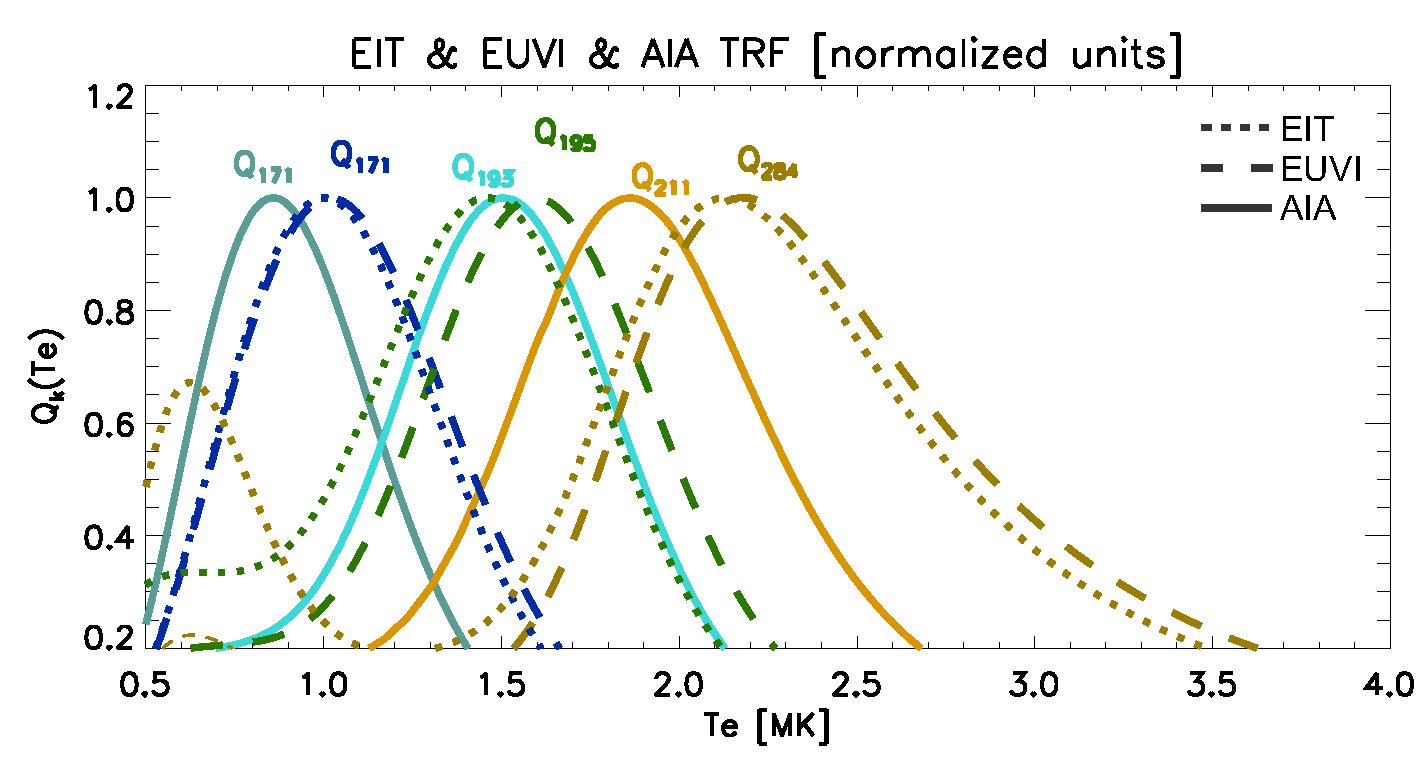
\includegraphics[height=0.56\textwidth]{figuras/qkl_aia_euvi_test_2.pdf}
%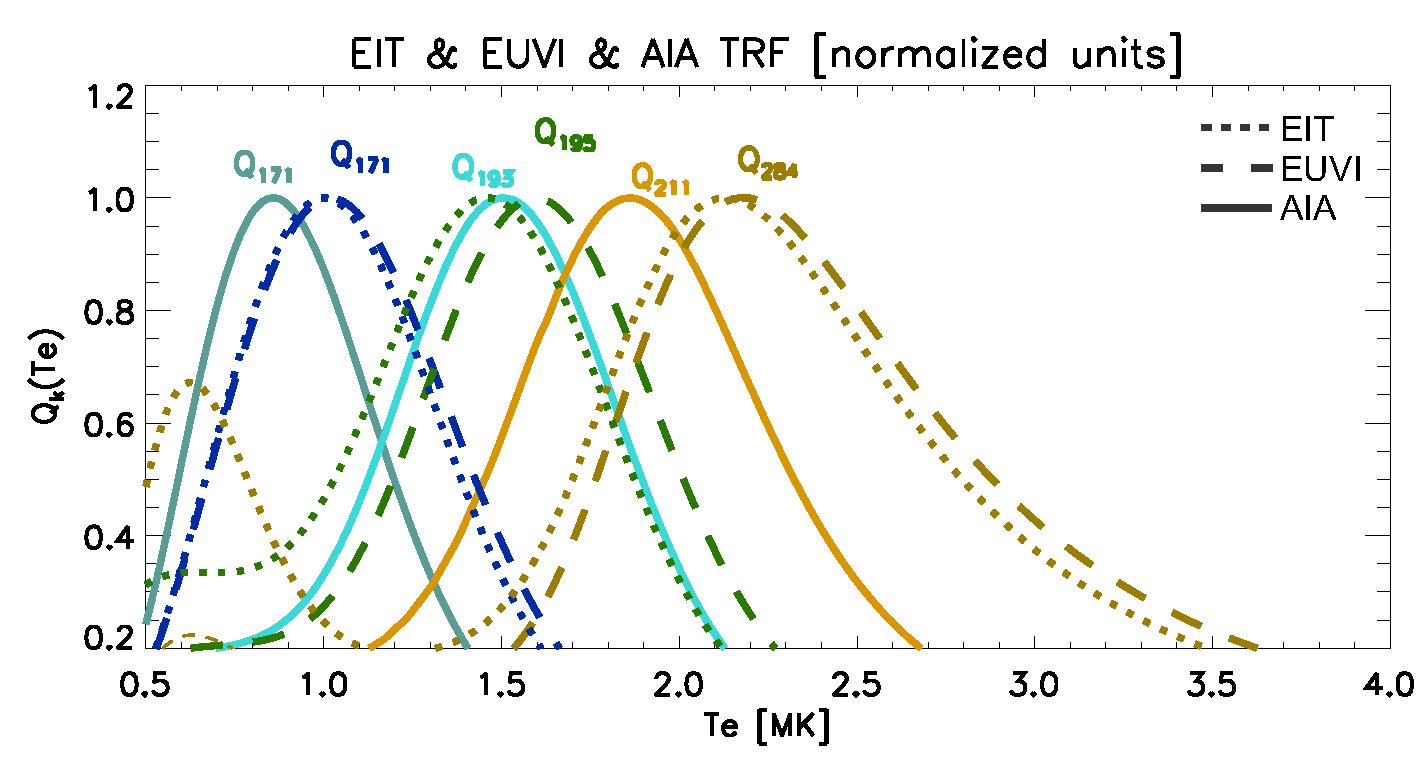
\includegraphics[width=0.99\textwidth]{figuras/qkl_aia_euvi_test_2.pdf}
%\end{columns}
%\end{comment}


$$
Q_k(T) \ \ \equiv \ \ \int {\rm d} \lambda \ \ \phi_k(\lambda) \ \ {\eta( N_{e0}, {\bf a}_0,
T; \lambda)} \ / \ {N_{e0}^2}
$$
\vskip 0.2cm
%\begin{columns}
%\column{0.3\textwidth}

%\column{0.7\textwidth}
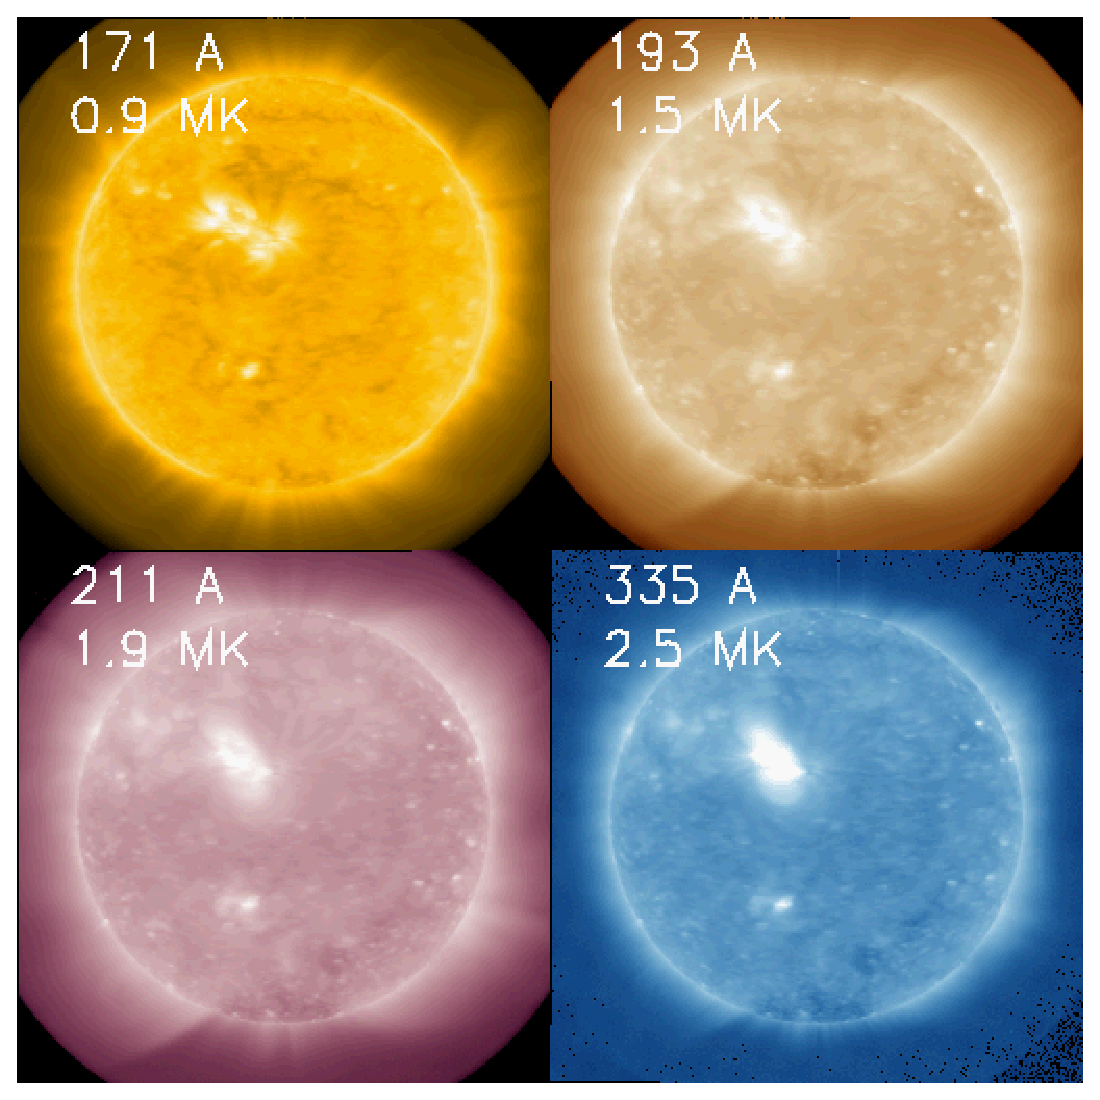
\includegraphics[height=0.32\linewidth,width=0.3\linewidth]{figuras/panel.eps}
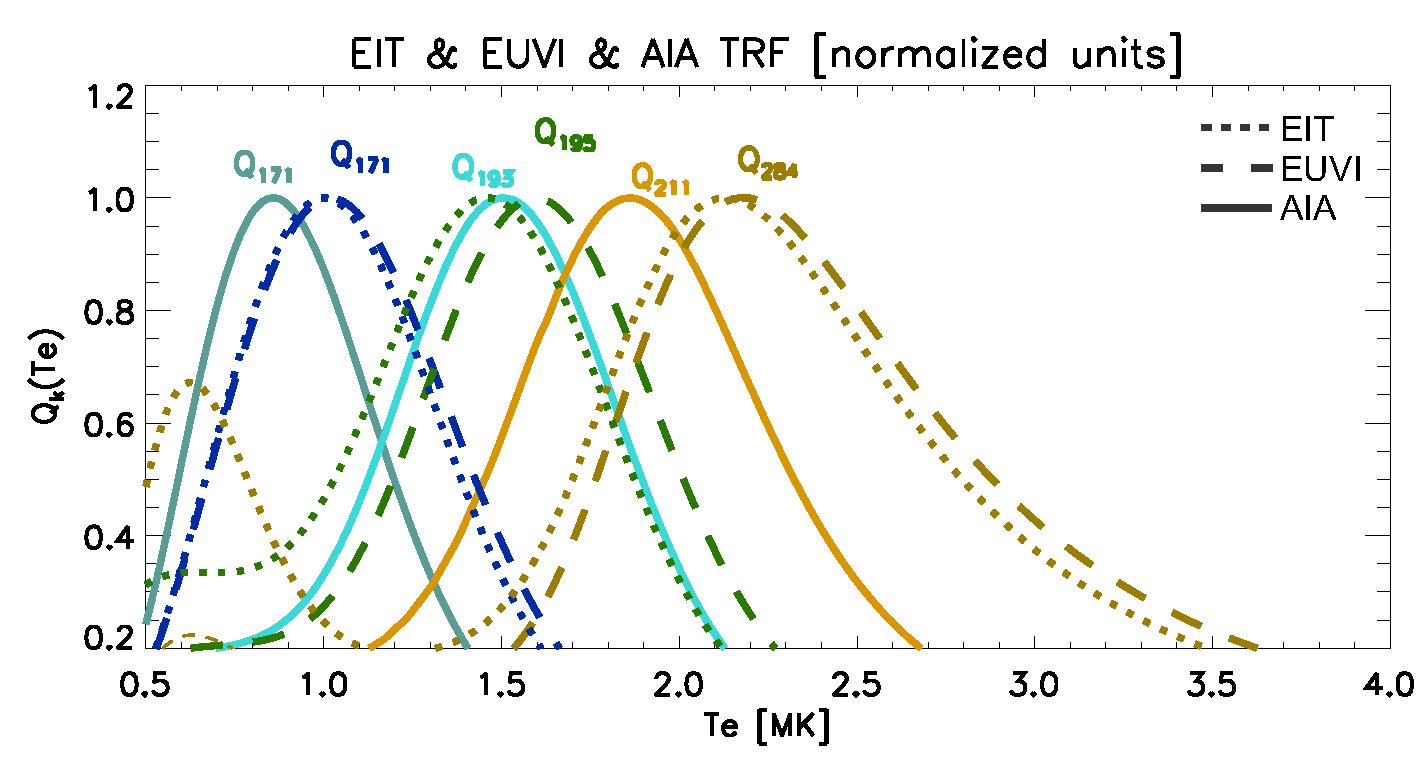
\includegraphics[height=0.35\textwidth,width=0.65\linewidth]{figuras/qkl_aia_euvi_test_2.pdf}
%\end{columns}

%\footnotesize
\bu $\phi_k$: Passband $k$ \hfill Lloveras et al. (2018)\\
%\vskip 0.25cm
\bu $\eta(\lambda,T,N)$: Spectral emissivity model.\\
Chianti v10, Del Zanna et al. (2021)
%\vskip 0.25cm
%\bu EUVI/EIT: ${\bf a}_0 =$ [Fe]\\
%Feldman et al. (1992)
}




%----------------------------------- LDEM

\begin{frame}%[noframenumbering]
\titulo{Local Differential Emission Measure (LDEM)}
\footnotesize
\begin{itemize}
\item
%En cada celda tomográfica \azul{$i$} se conocen K \azul{FBEs}.
For each band \azul{$k$} we now know the \azul{FBE$_{k,i}$} at each tomographic voxel \azul{$i$}.
\salto
%\item
%Utilizando las Respuestas Térmicas \azul{$Q_k(T)$}
%\salto
\item
The FBEs can be re-written as:
$\azul{FBE_{k,i} } \, = \, \azul{\int \mathrm{d}T \  Q_k(T) \ \, \rojo{{\sf LDEM}_i(T)} }$.
\salto
\item
Where the \rojo{${\sf LDEM}_i(T)$ [cm$^{-6}$K$^{-1}$]} of each voxel \azul{$i$} is defined so that:
\begin{eqnarray}
N_{m,i}^2 = \left< N_e^2\right>_i &=& \int \mathrm{d} T \ \, \rojo{{\sf LDEM}_i(T)}\nonumber\\
T_{m,i} = \left<T_e\right>_i  &=& \frac{1}{\left< N_e^2\right>_i } \int \mathrm{d}T\ T \ \, \rojo{{\sf LDEM}_i(T)}\nonumber \\
 W_{T,i}^2 &=&  \frac{1}{\left< N_e^2\right>_i} \int_{T_{min}}^{T_{max}} dT\ \rojo{{\sf LDEM}_i(T)}\ (T - \langle T_e \rangle_i)^2 \nonumber
\end{eqnarray}
%\salto
\item A parametric model for the LDEM is chose:\ 
$\rojo{{\sf LDEM}_i(T)}=\azul{\mathcal{N}(}T,\,\rojo{\mathbf{\lambda}_i=[A,T_0,\sigma_T]}\azul{)}$ Nuevo et al. (2015)
\salto
\item
The following cost function is minimized in each cell: \mediosalto
\hskip 3cm
$
\Phi(\rojo{{\mathbf{\lambda}}_i}) \ = \ 
\ \azul{\sum_{k}}| \ \azul{ FBE_{k,i} }-
\azul{\int \mathrm{d}T \ \, Q_k(T)\ \, \mathcal{N}(T,}\,\rojo{\mathbf{\lambda}_i}\azul{)} \ 
|^2 
$.
\item Succes rate 
$
R_i \equiv (1/K) \sum_{k} | 1 - { FBE_{k,i} } / {\int \mathrm{d}T \ \, Q_k(T)\ \, \mathcal{N}(T,}\,{\mathbf{\lambda}_i}{)} |
$
\end{itemize}
\end{frame}


%--------------------------
\begin{frame}[noframenumbering]
\titulo{Typical LDEM}
\begin{center}
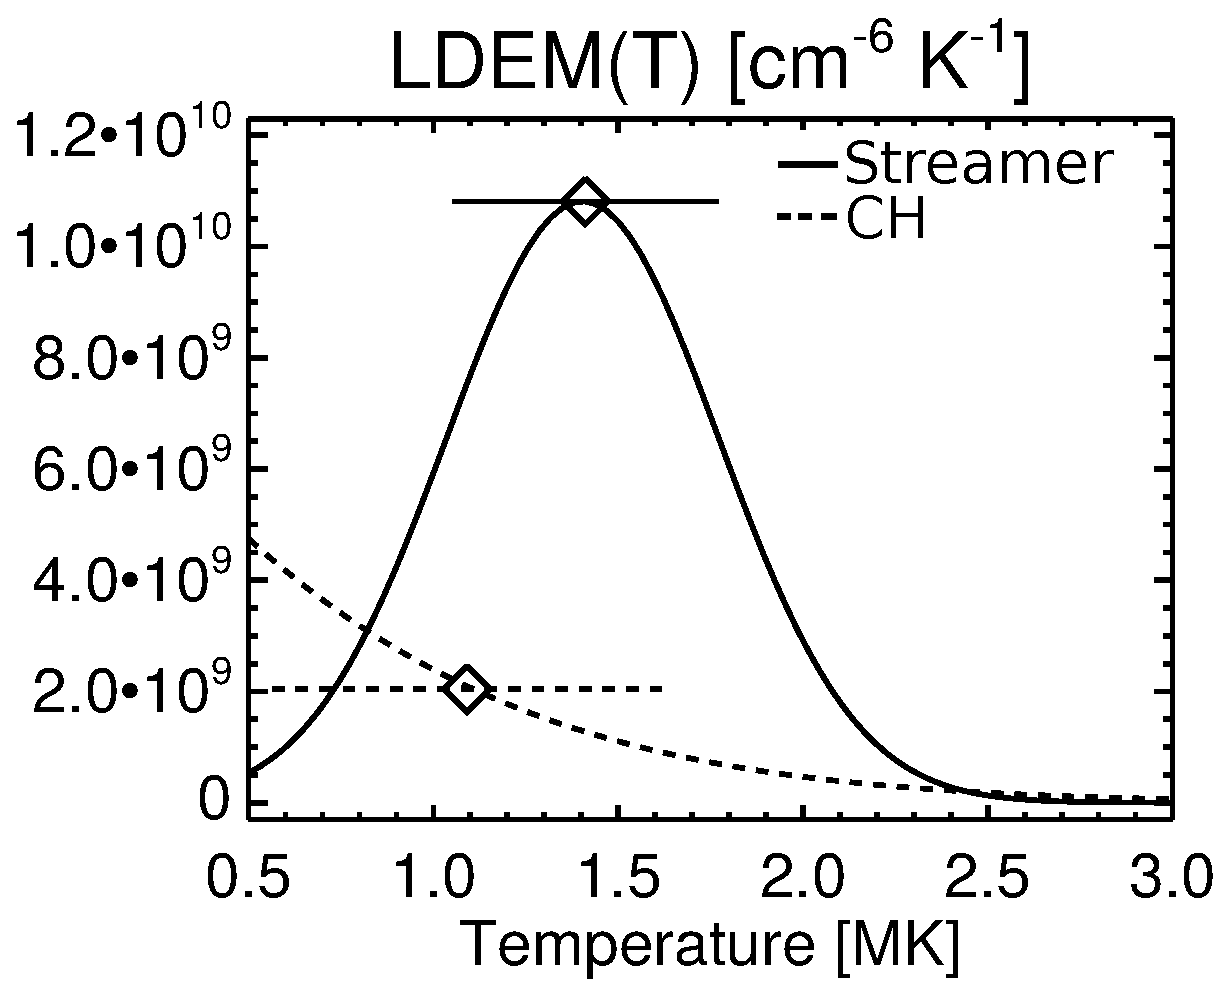
\includegraphics[width=0.495\textwidth,clip=]{figuras/Nueva_figura_paper_LDEM_2.eps}
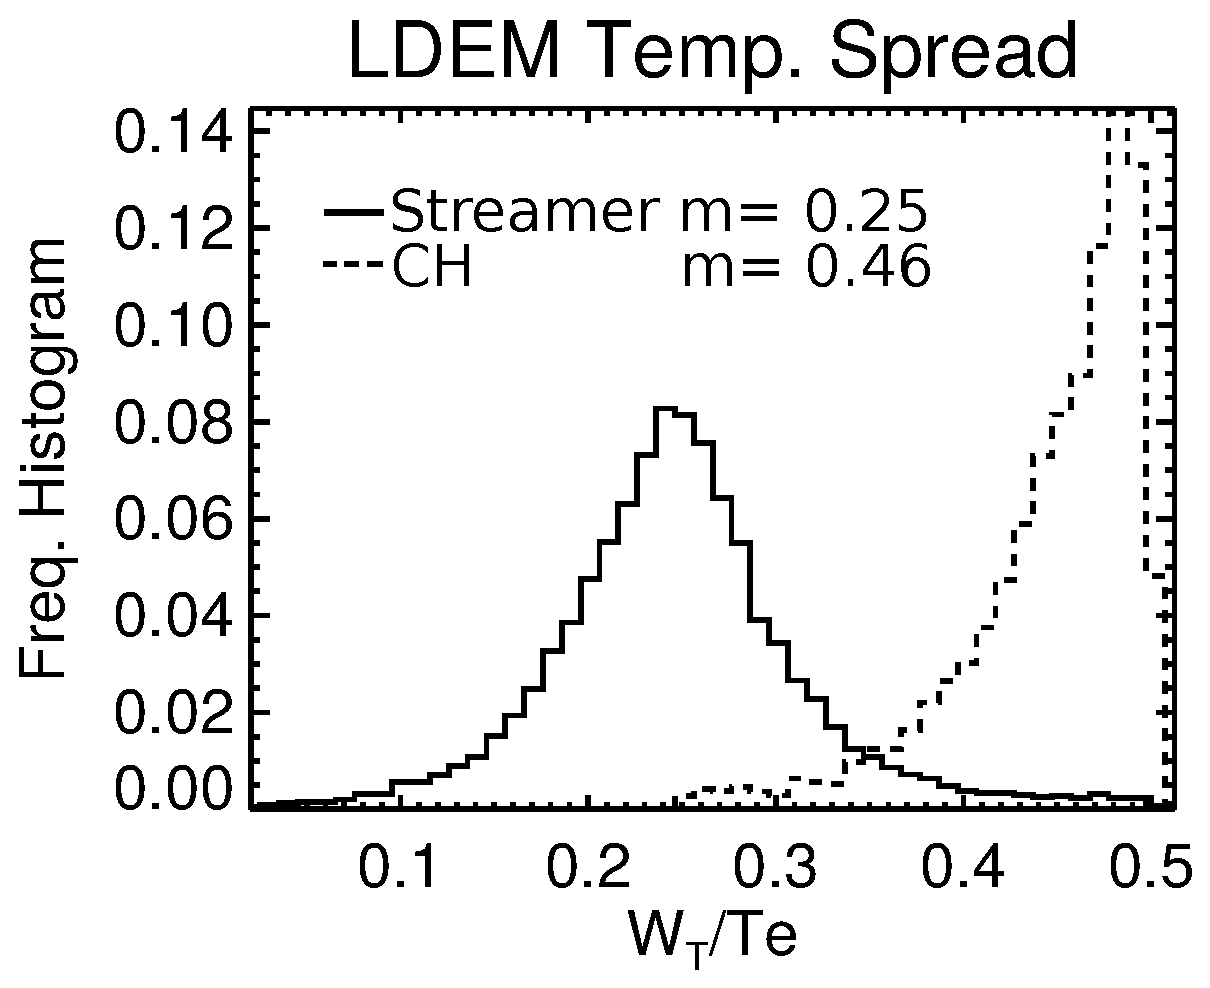
\includegraphics[width=0.495\textwidth,clip=]{figuras/Nueva_figura_paper_3.eps}
\end{center}

\begin{columns}
  
\column{0.5\textwidth}
%Lloveras et al. (2022)
\begin{center}
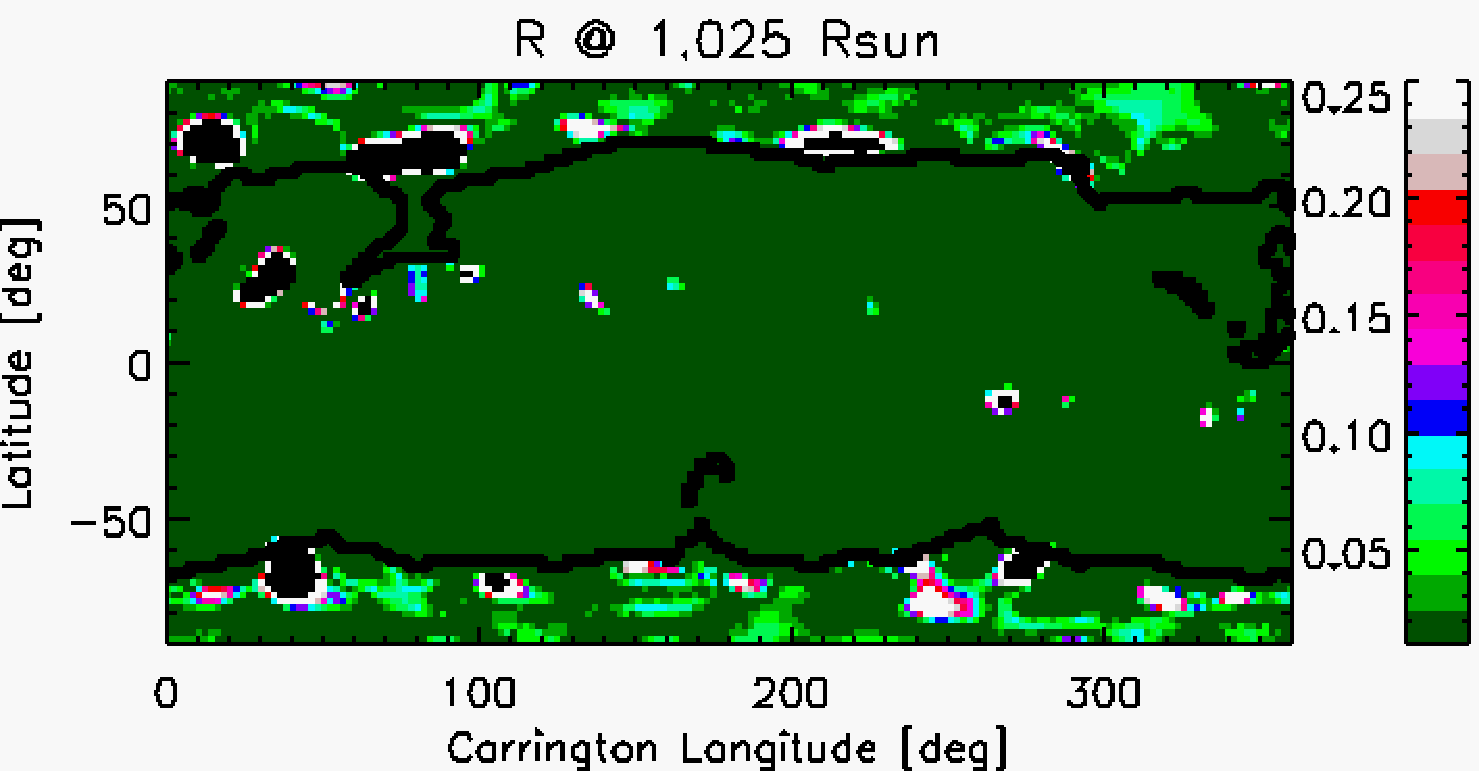
\includegraphics[width=0.99\textwidth,clip=]{figuras/R_1025_CR2081.pdf}
\end{center}

\column{0.5\textwidth}
\hfill Lloveras et al. (2022)\\

\vskip 2cm
$R \sim 1\% \, (Streamer) \, y \sim 10\% \, (CHs)$

\end{columns}
\end{frame}

%-----------------------------------------------------------

%{
%\setbeamercolor{title}{fg=blue}
%\setbeamercolor{normal text}{fg=black}
%\setbeamercolor{frametitle}{fg=blue}
%\usebeamercolor[fg]{normal text}
%\usebackgroundtemplate{{\includegraphics[width=\paperwidth]
%{figuras/fondo_poster_70x90cm.pdf}}}
%\frame{
%\titulo{The Solar cycle and the Coronal Activity}
%\footnotesize

%\begin{columns}
%\column{0.5\textwidth}
%\begin{center}
%Babcock et al. (1961)\\
%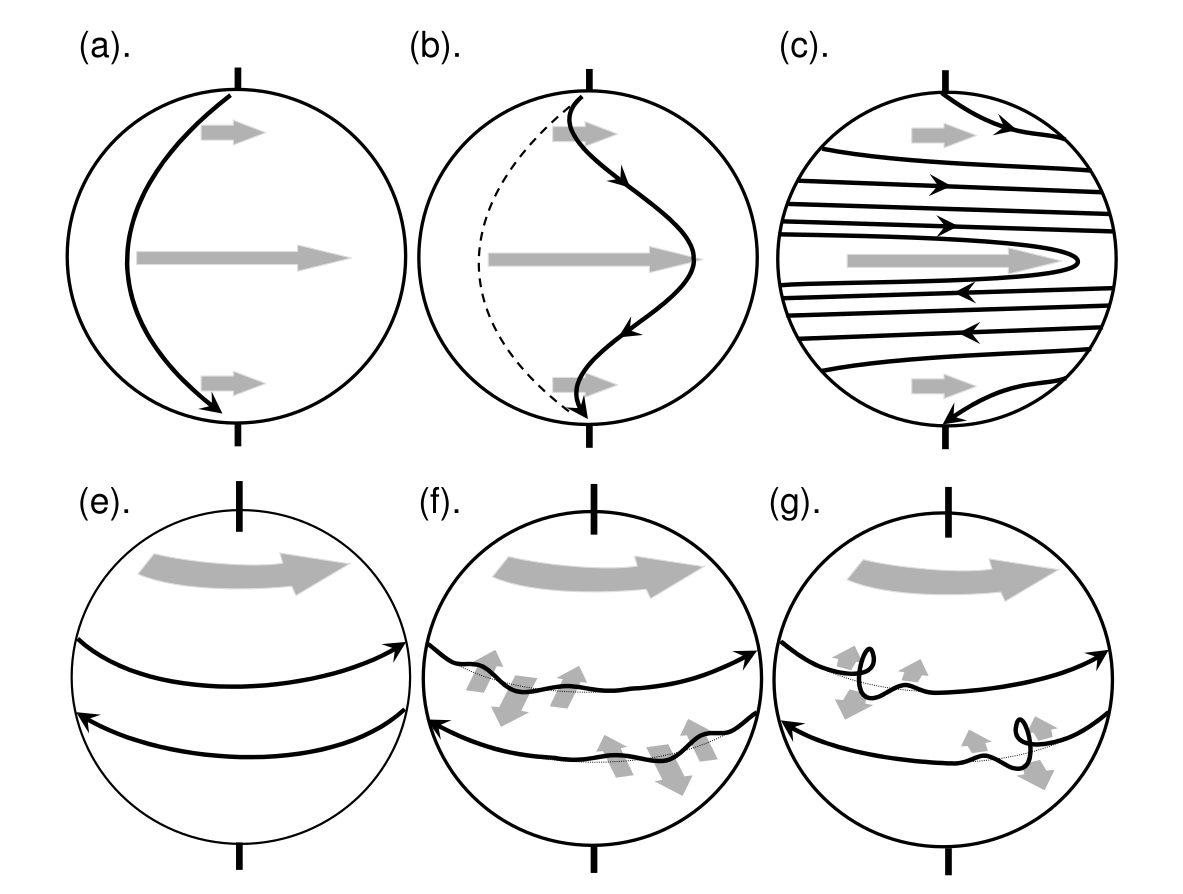
\includegraphics[width=0.7\textwidth]{figuras/babckok_model.png}
%Landi et al. (2016)\\
%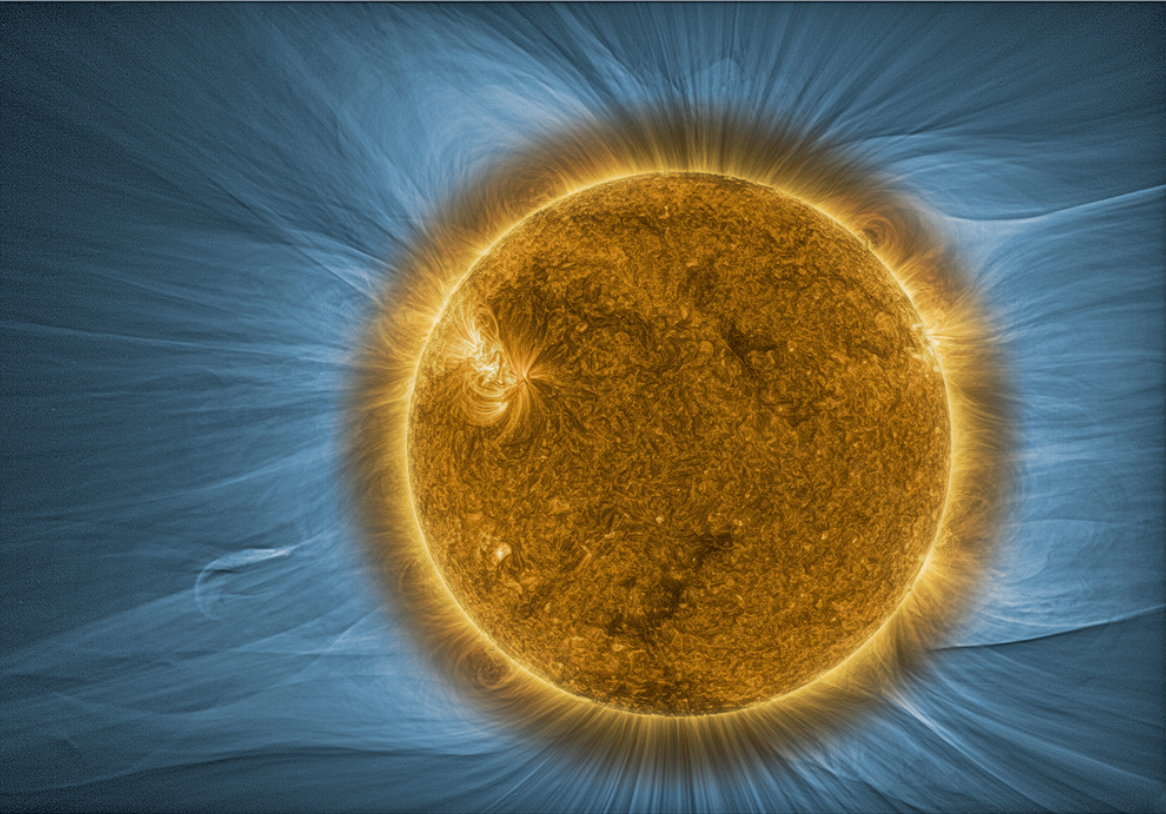
\includegraphics[width=0.6\textwidth,height=0.5\textwidth]{figuras/landi.png}
%\end{center}
%\column{0.5\textwidth}
%\begin{center}
%\bu Solar dynamo $\rightarrow$ B(t).\\
%\vskip 0.5cm
%\bu Mínima: Global dipolo, few SSs/ARs.\\
%\vskip 0.5cm
%\bu Maxima: Multipole, many SSs/ARs.\\
%\vskip 0.5cm
%\bu Period $\sim$ 11 years\\

%\end{columns}


%\vspace{-0.55cm}
%\begin{center}
%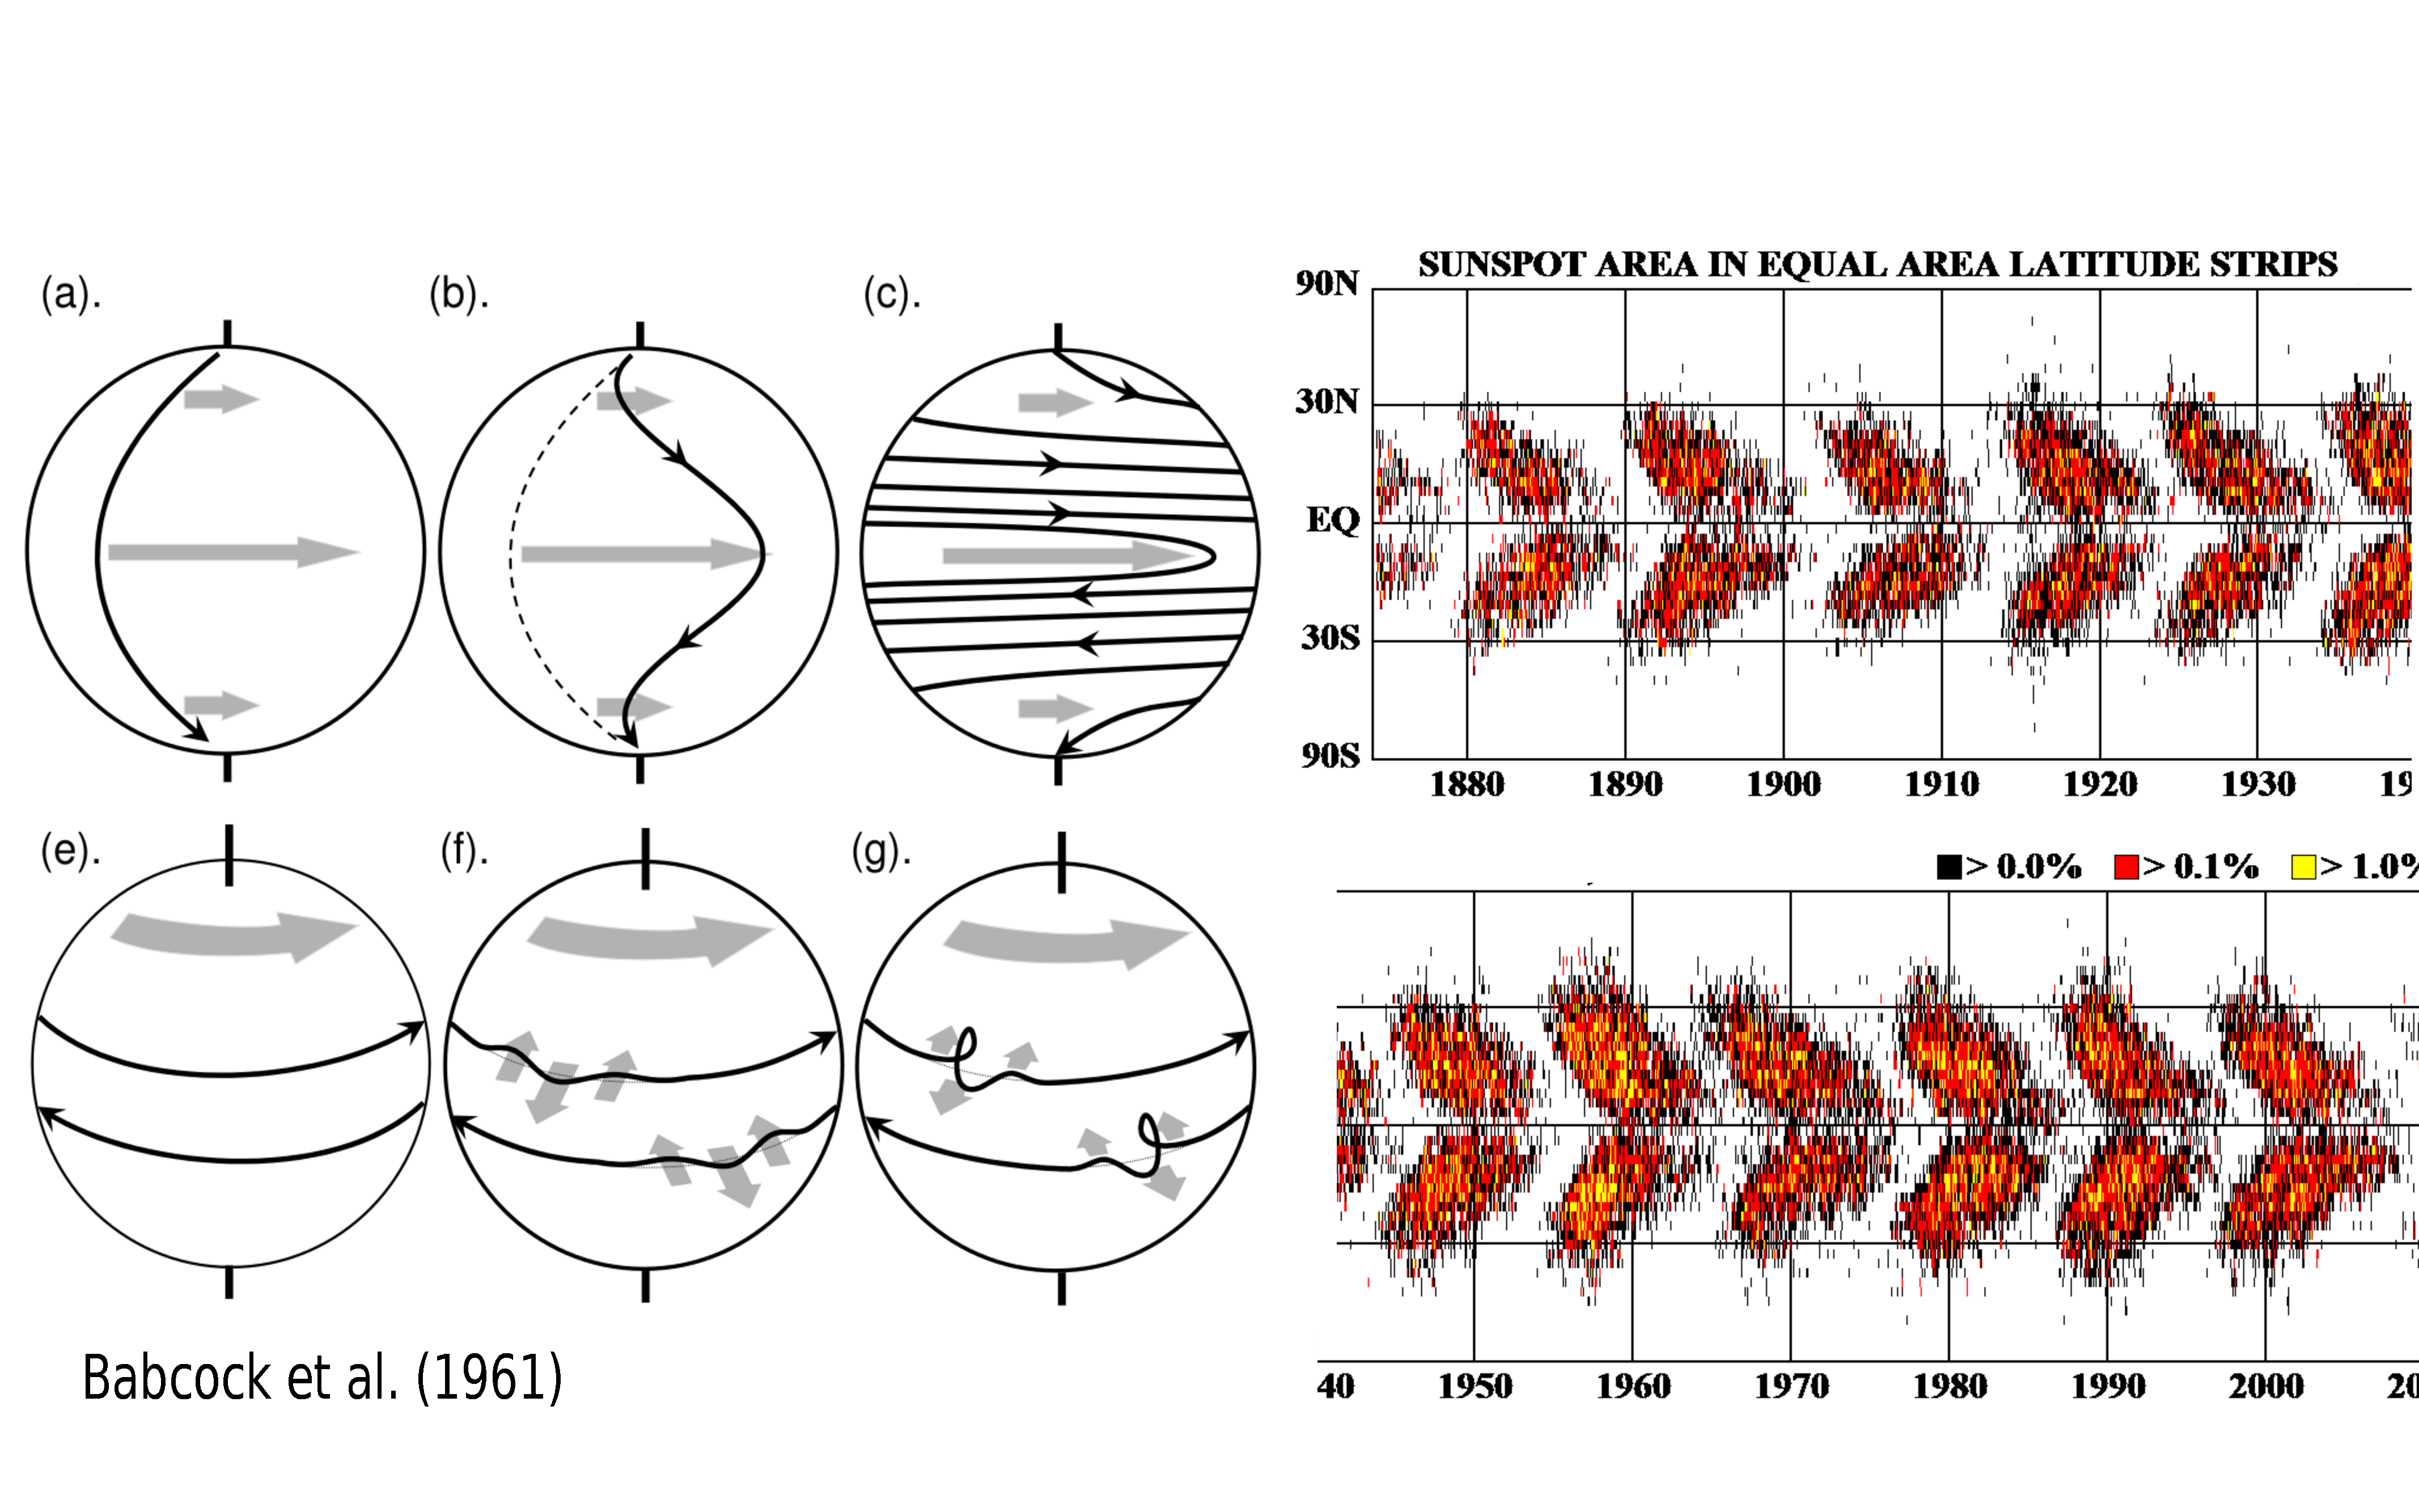
\includegraphics[width=.6\textwidth]{figuras/butterfly-diagram_recorte.pdf}
%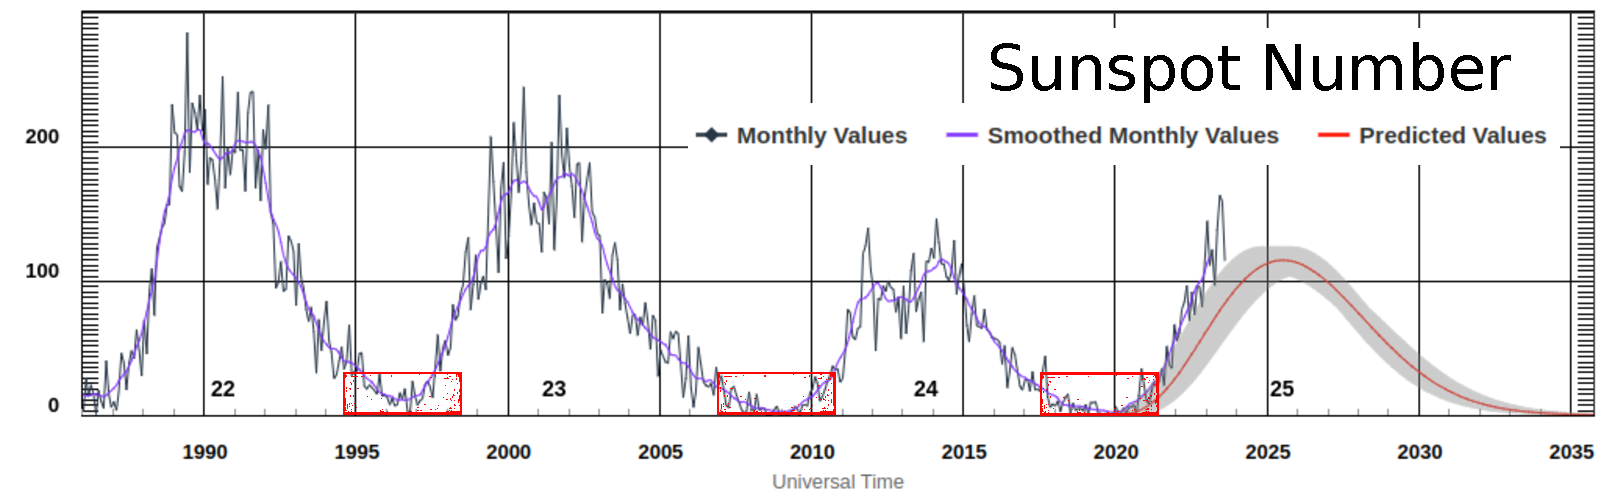
\includegraphics[width=0.99\textwidth]{figuras/conteo_manchas_full.pdf}
%\end{center}
%\vskip -0.5cm
%Space weather prediction center (NOAA)
%}
%}













%-------------------------------SRT
%{
%\setbeamercolor{title}{fg=blue}
%\setbeamercolor{normal text}{fg=black}
%\setbeamercolor{frametitle}{fg=blue}
%\usebeamercolor[fg]{normal text}
%\usebackgroundtemplate{{\includegraphics[width=\paperwidth]
%{figuras/fondo_poster_70x90cm.pdf}}}
%\frame{
%\titulo{Solar Rotational Tomography (SRT)}
%\footnotesize
%\vspace*{-0.25cm}
%\begin{center}
%{\bf
%The object of study is the Solar Corona.\\
%Solar rotation and telescope's orbit provide the multiple viewpoints.
%}
%\end{center}
%\vspace{-1.cm}
%\begin{columns}
%\vspace{-1cm}
%\column{0.65\textwidth}
%\ \ 
%\vskip 0.5cm
%\begin{itemize}
%\item[\bu] 
%\azul{Corona-K:} Thomson scatt. of photosph. \azul{WL} $\rightarrow$\\
%diagnostic of coronal $\Ne$.
%\item[\bu] \azul{SRT-WL} $\rightarrow$ 3D $\Ne$.  \hfill C2-SRT $2.5 - 6.5 \mrsun$
%\item[\bu] {1st SRT-WL: Altschuler \& Perry (1972)}
%\end{itemize}
%\vskip 1cm
%\begin{itemize}
%\item[\bu] \azul{Corona-E:} coll-excited \azul{EUV} coronal emission $\rightarrow$\\
%diagnostic of coronal $\Ne$ and $\Te$.
%\item[\bu] \azul{SRT-EUV} $\rightarrow$ 3D EUV emissivity  $\rightarrow$\\
%3D Differential Emission Measure $\rightarrow$\\
%3D $\Ne$ y $\Te$. \hfill EUV-SRT $1.0 - 1.3 \mrsun$
%\item[\bu] {1st SRT-EUV and \azul{DEM-Tomography}:\\ 
%Vásquez, Frazin \& Kamalabadi (2009)\\
%Frazin, Vásquez \& Kamalabadi (2009)}
%\end{itemize}
%\column{0.4\textwidth}
%\vskip 1cm
%\begin{center}
%\azul{White Light Coronagraph}\\
%\figu{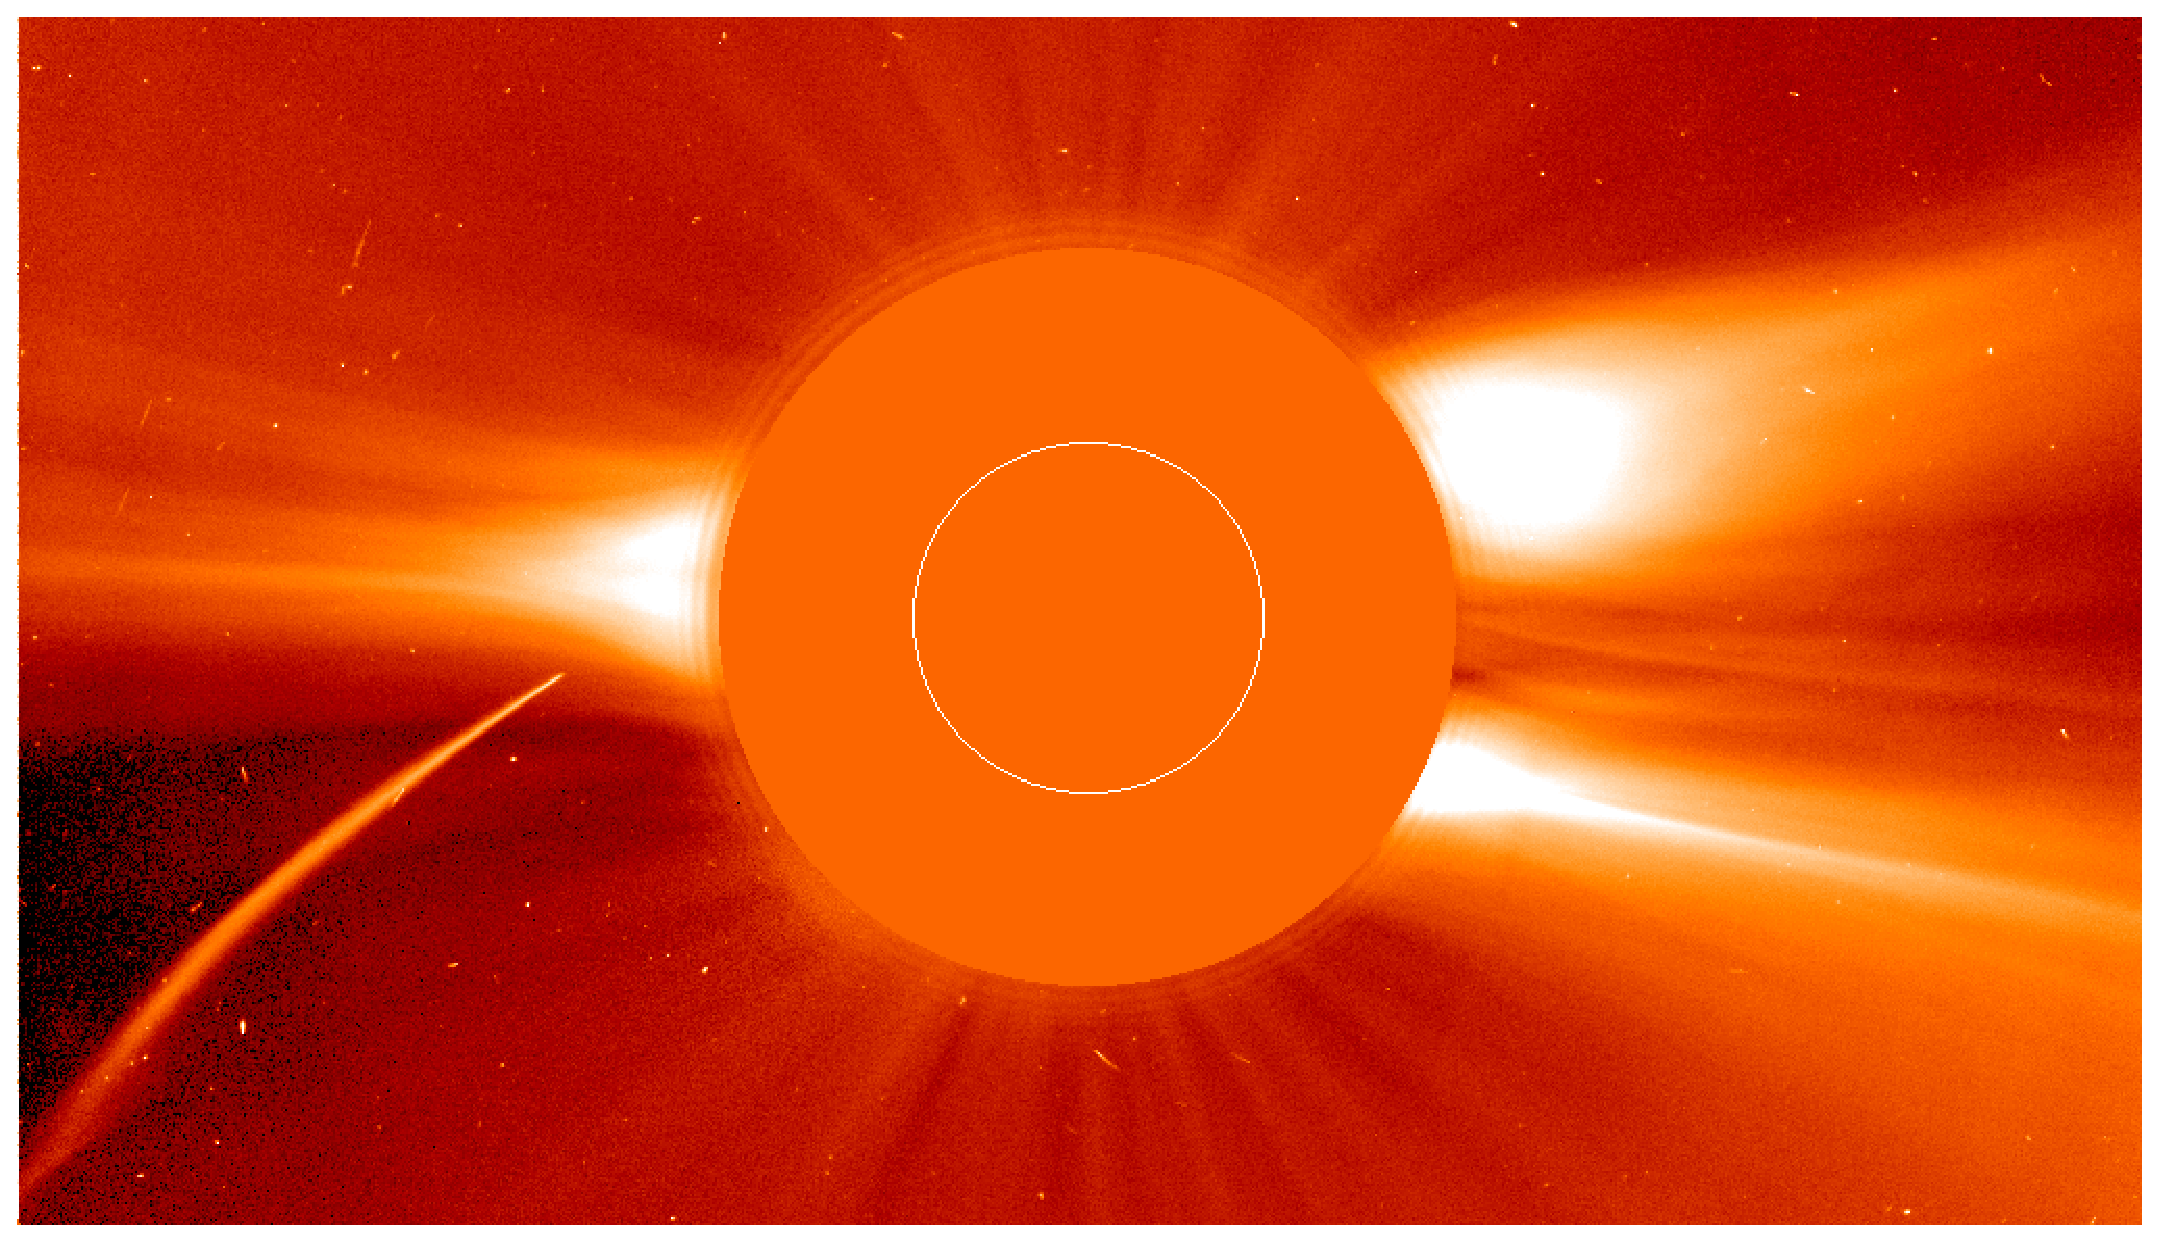
\includegraphics[width=0.7\textwidth]{figuras/LASCOC2_comet.eps}}
%\mediosalto
%\azul{EUV Telescope}\\
%\figu{\includegraphics[width=0.7\textwidth]{figuras/aia_211_fullsun.eps}}
%\end{center}
%\end{columns}
%}
%}
%--------------- Carrmaps
{
\setbeamercolor{title}{fg=blue}
\setbeamercolor{normal text}{fg=black}
\setbeamercolor{frametitle}{fg=blue}
\usebeamercolor[fg]{normal text}
\usebackgroundtemplate{{
\includegraphics[width=\paperwidth]
{figuras/fondo_poster_70x90cm.pdf}}}
\frame{
\titulo{EUV-SRT Comparative Solar Minima Study}
\begin{columns}
\column{0.35\textwidth}
\centering
CR-1915 (EIT)
\vskip 0.3cm
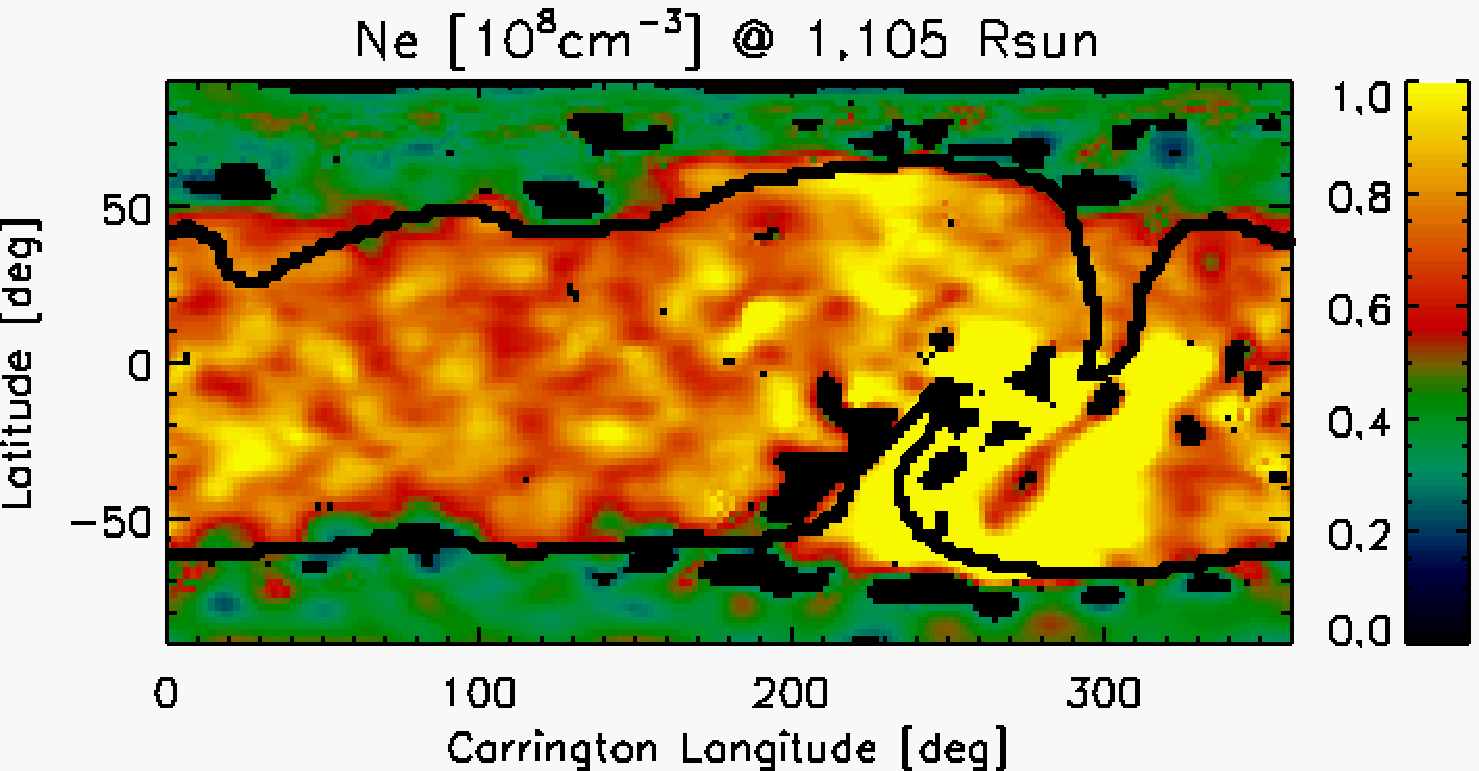
\includegraphics[width=0.95\textwidth,clip=]{figuras/Ne_1105_CR1915.pdf}
\vskip 0.1cm
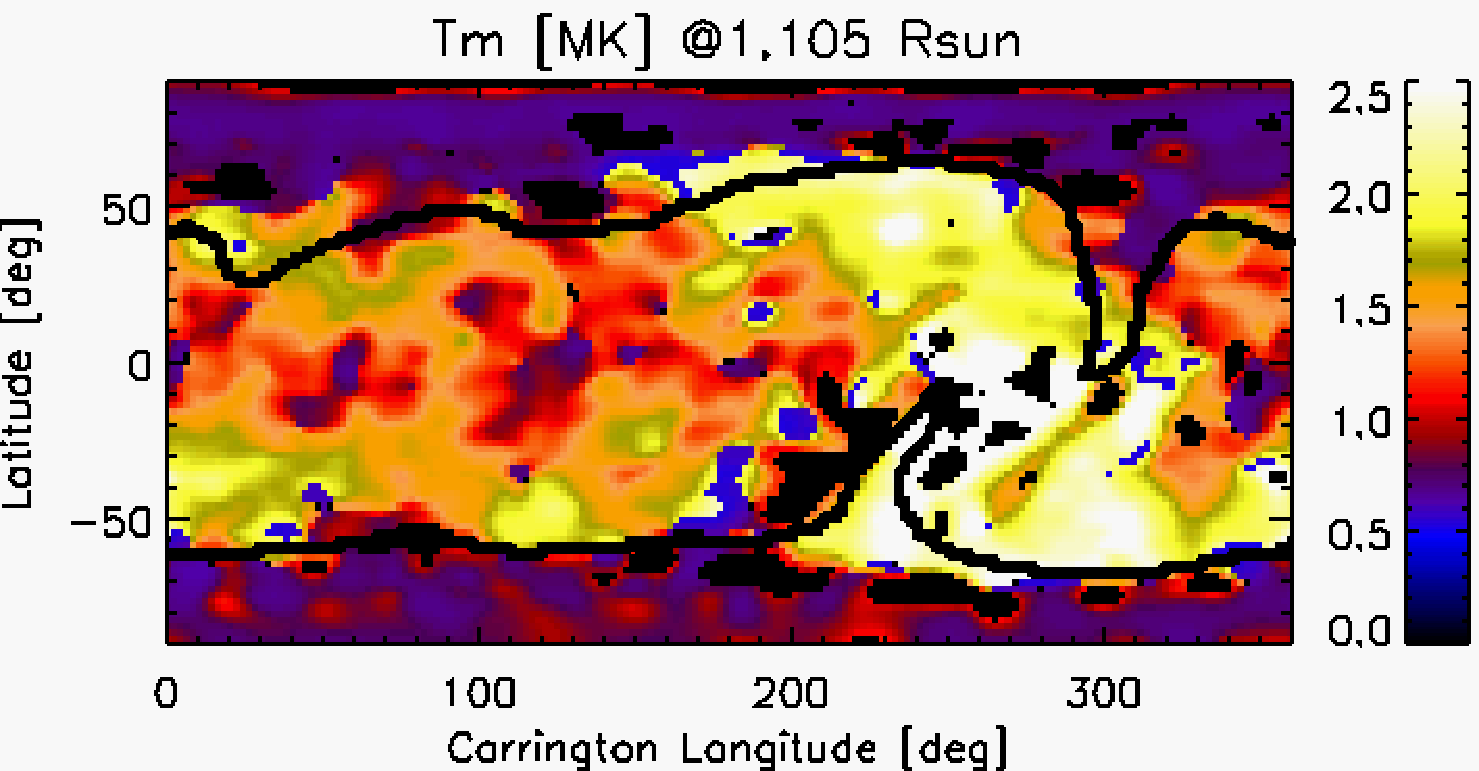
\includegraphics[width=0.95\textwidth,clip=]{figuras/Tm_1105_CR1915.pdf}

\column{0.35\textwidth}
\centering
CR-2081 (EUVI)
\vskip 0.3cm
%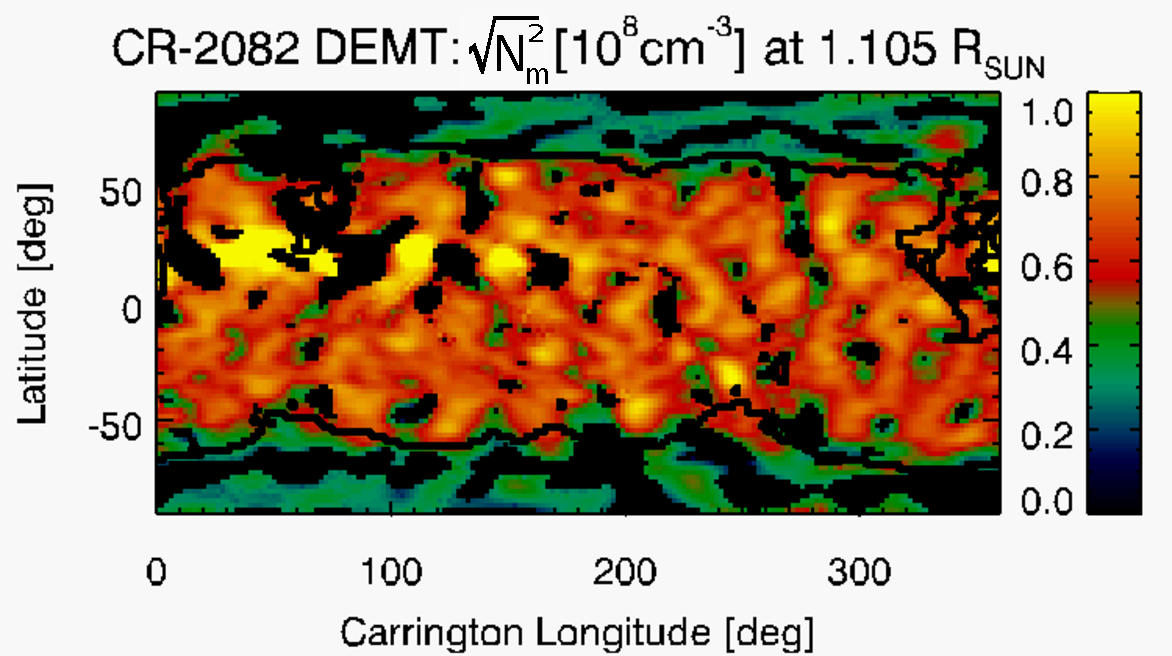
\includegraphics[width=0.95\textwidth]{figuras/map_Ne_CR2082_DEMT-EUVI_behind_H1-L3523_r3d_1105_Rsun.pdf}
%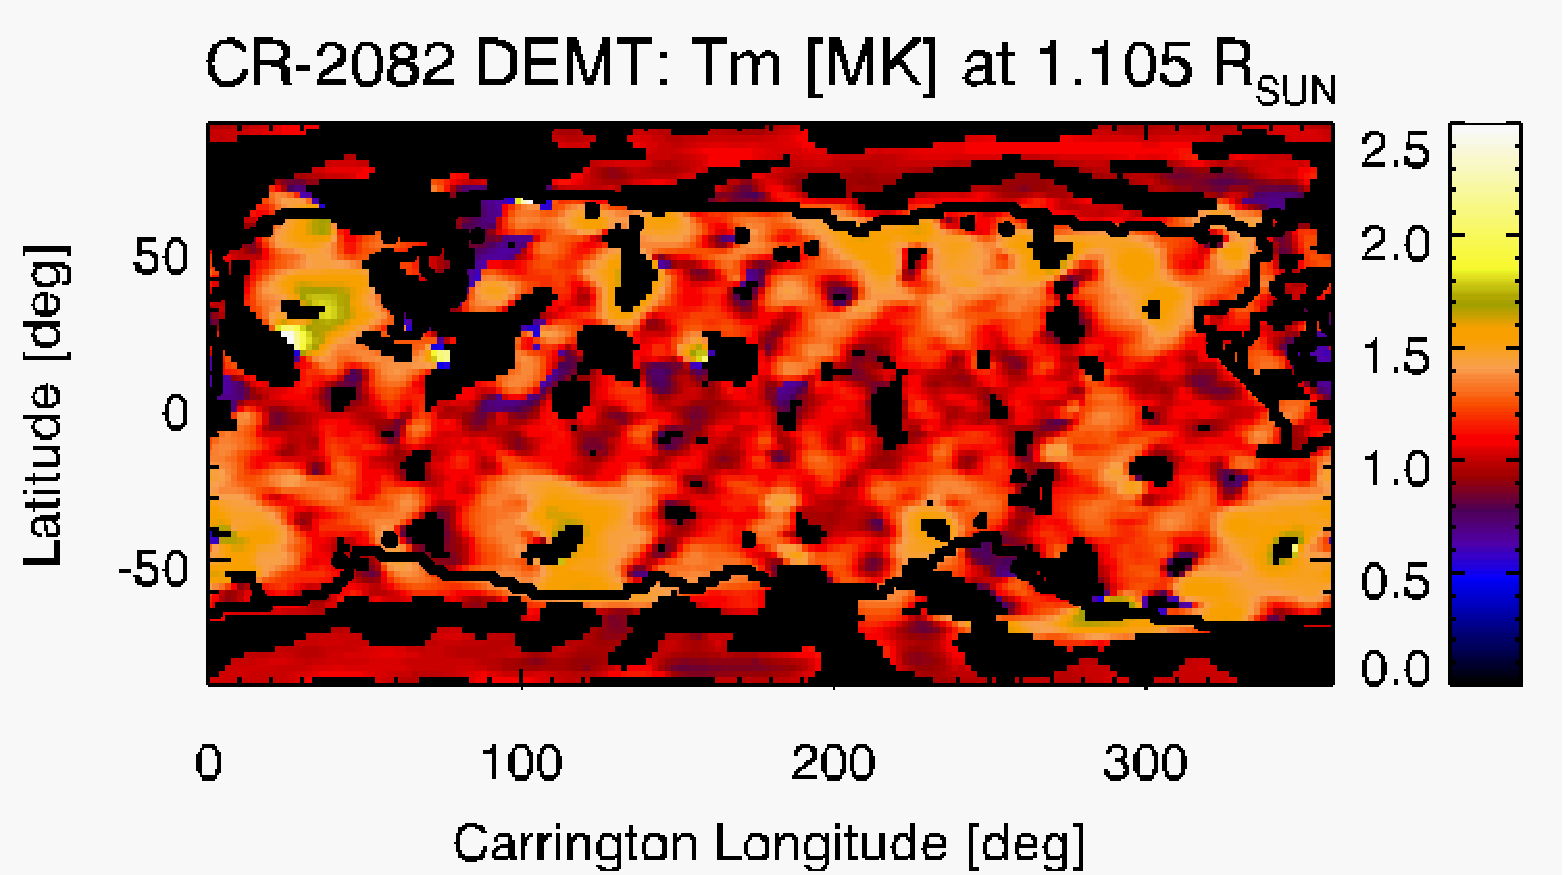
\includegraphics[width=0.95\textwidth]{figuras/map_Tm_CR2082_DEMT-EUVI_behind_H1-L3523_r3d_1105_Rsun.pdf}
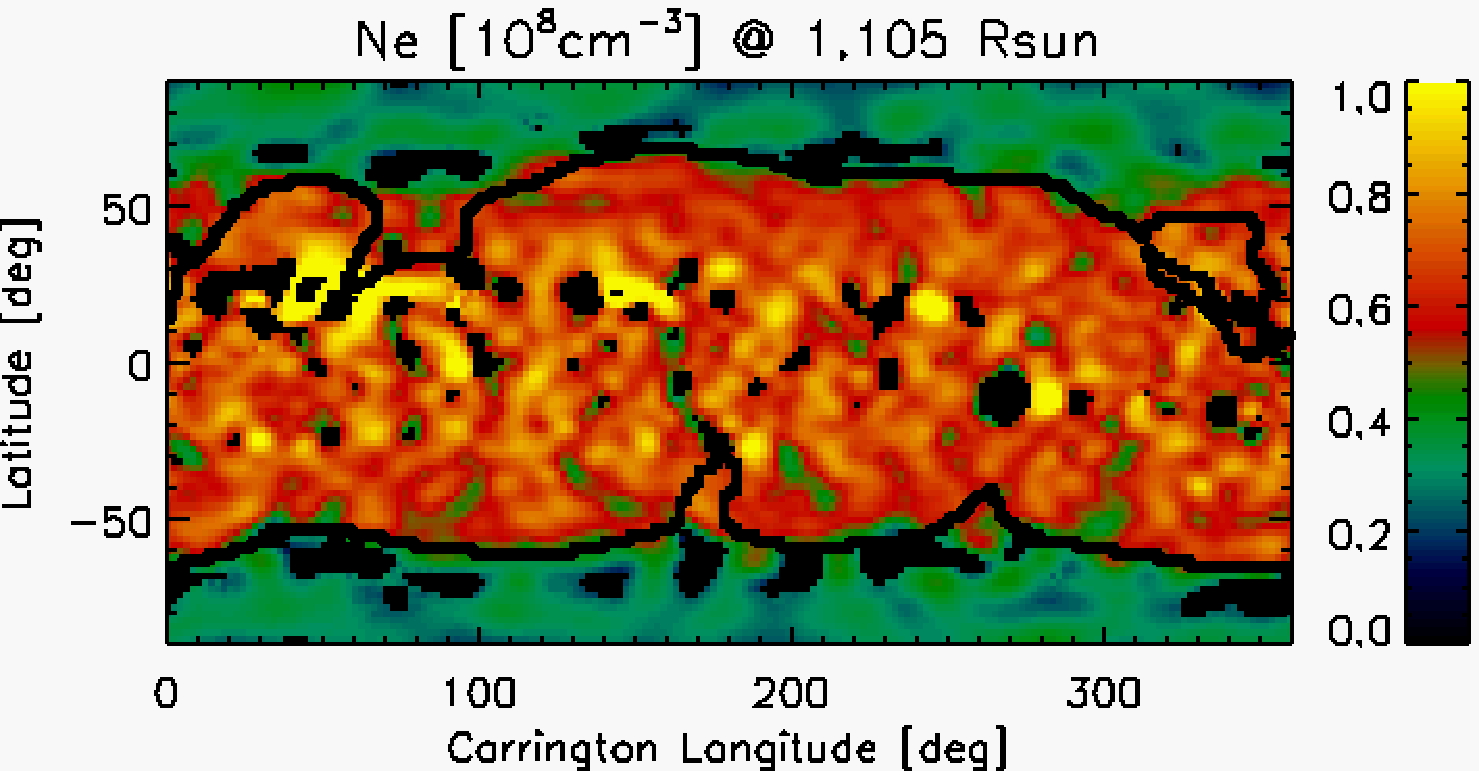
\includegraphics[width=0.95\textwidth]{figuras/Ne_1105_CR2081.pdf}
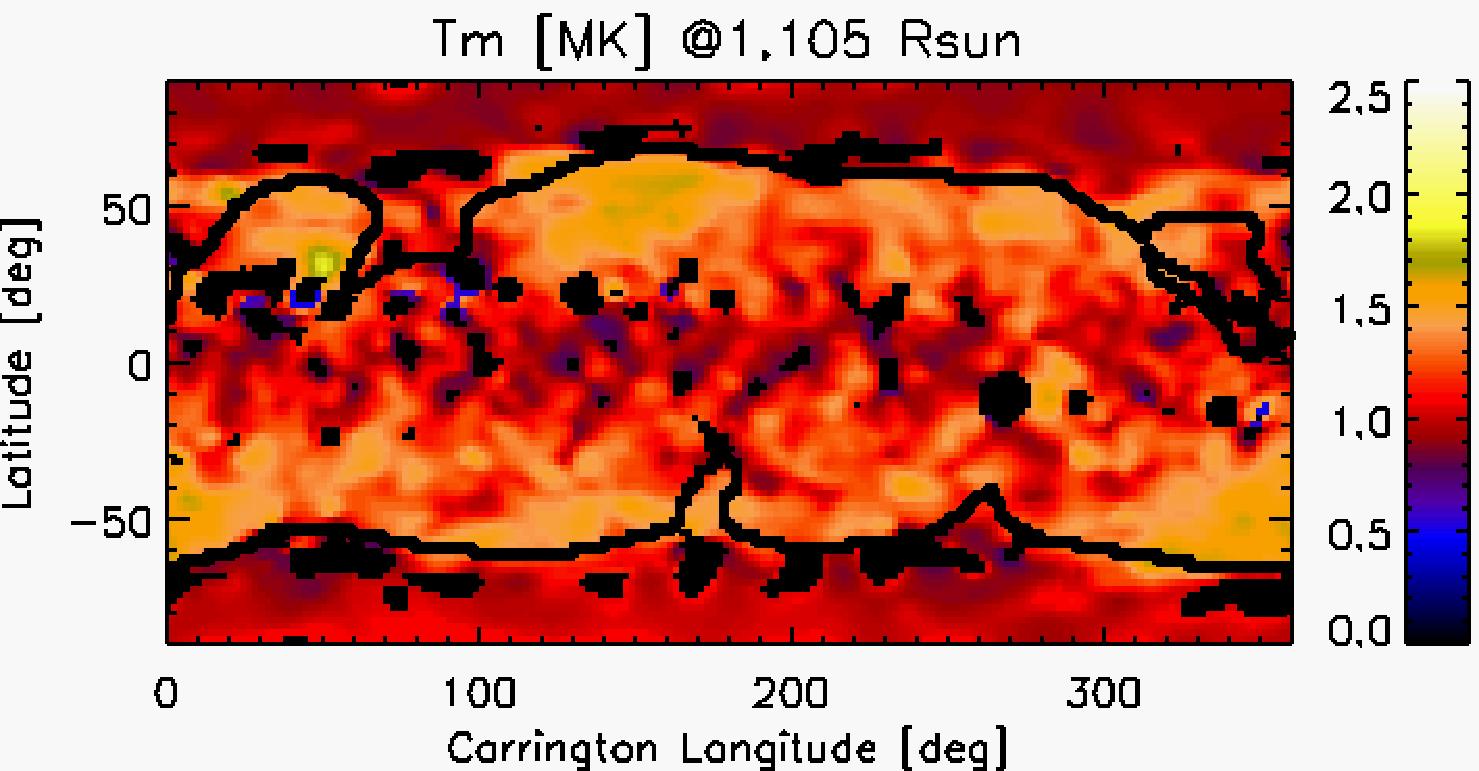
\includegraphics[width=0.95\textwidth]{figuras/Tm_1105_CR2081.pdf}

\column{0.35\textwidth}
\centering
CR-2223 (AIA)
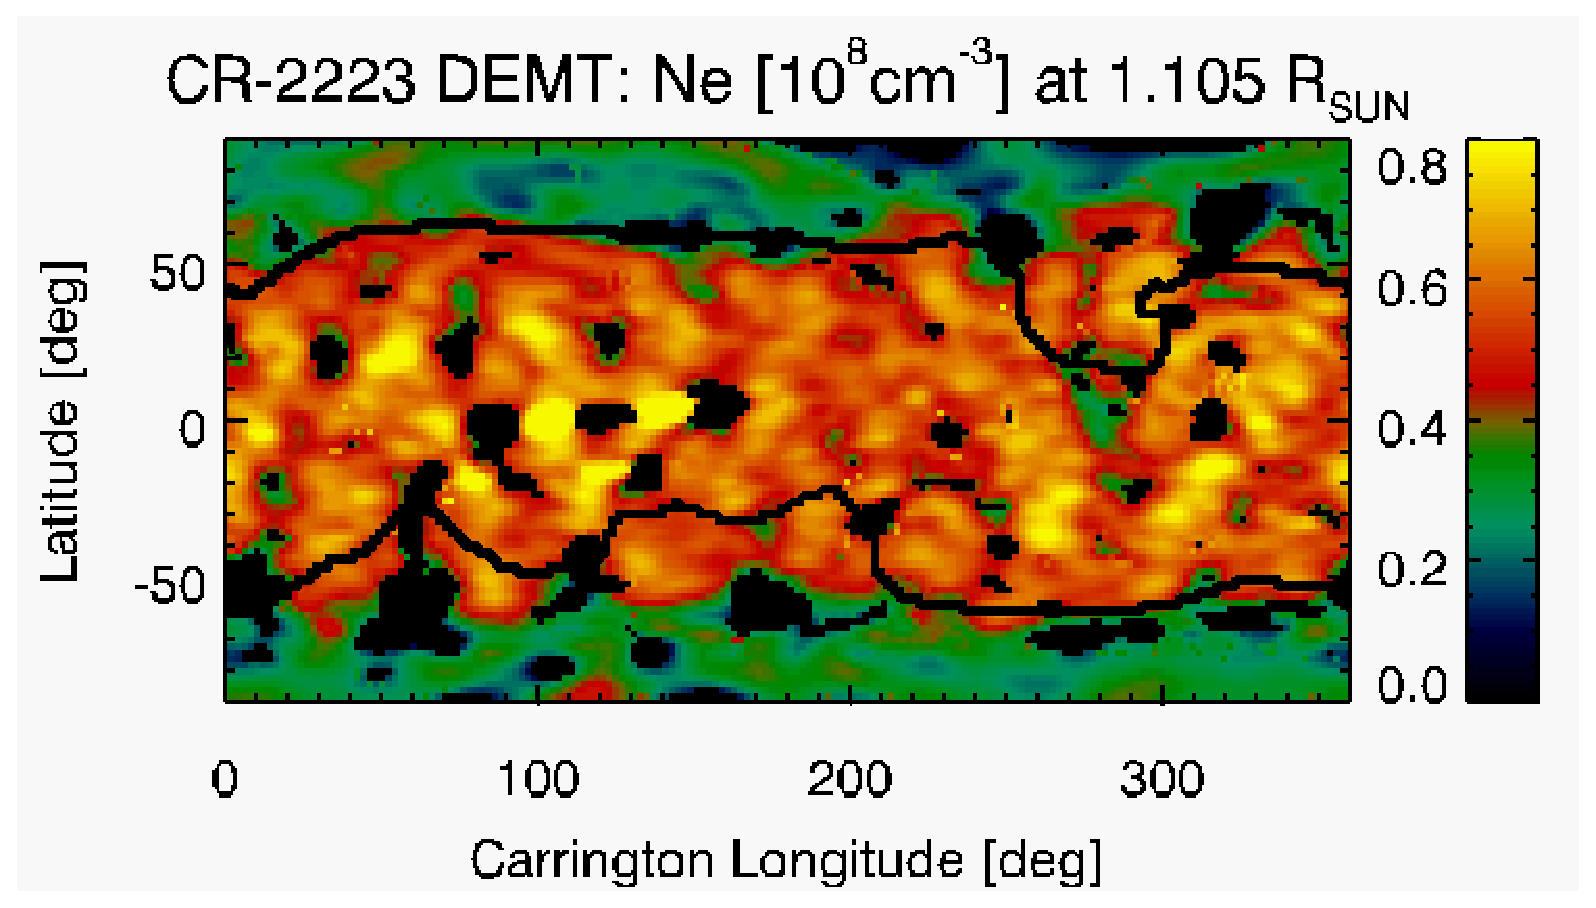
\includegraphics[width=0.95\textwidth,clip=]{figuras/map_Ne_CR2223_DEMT-AIA_H1_L733_r3d_multistart_1105_Rsun2223.eps}
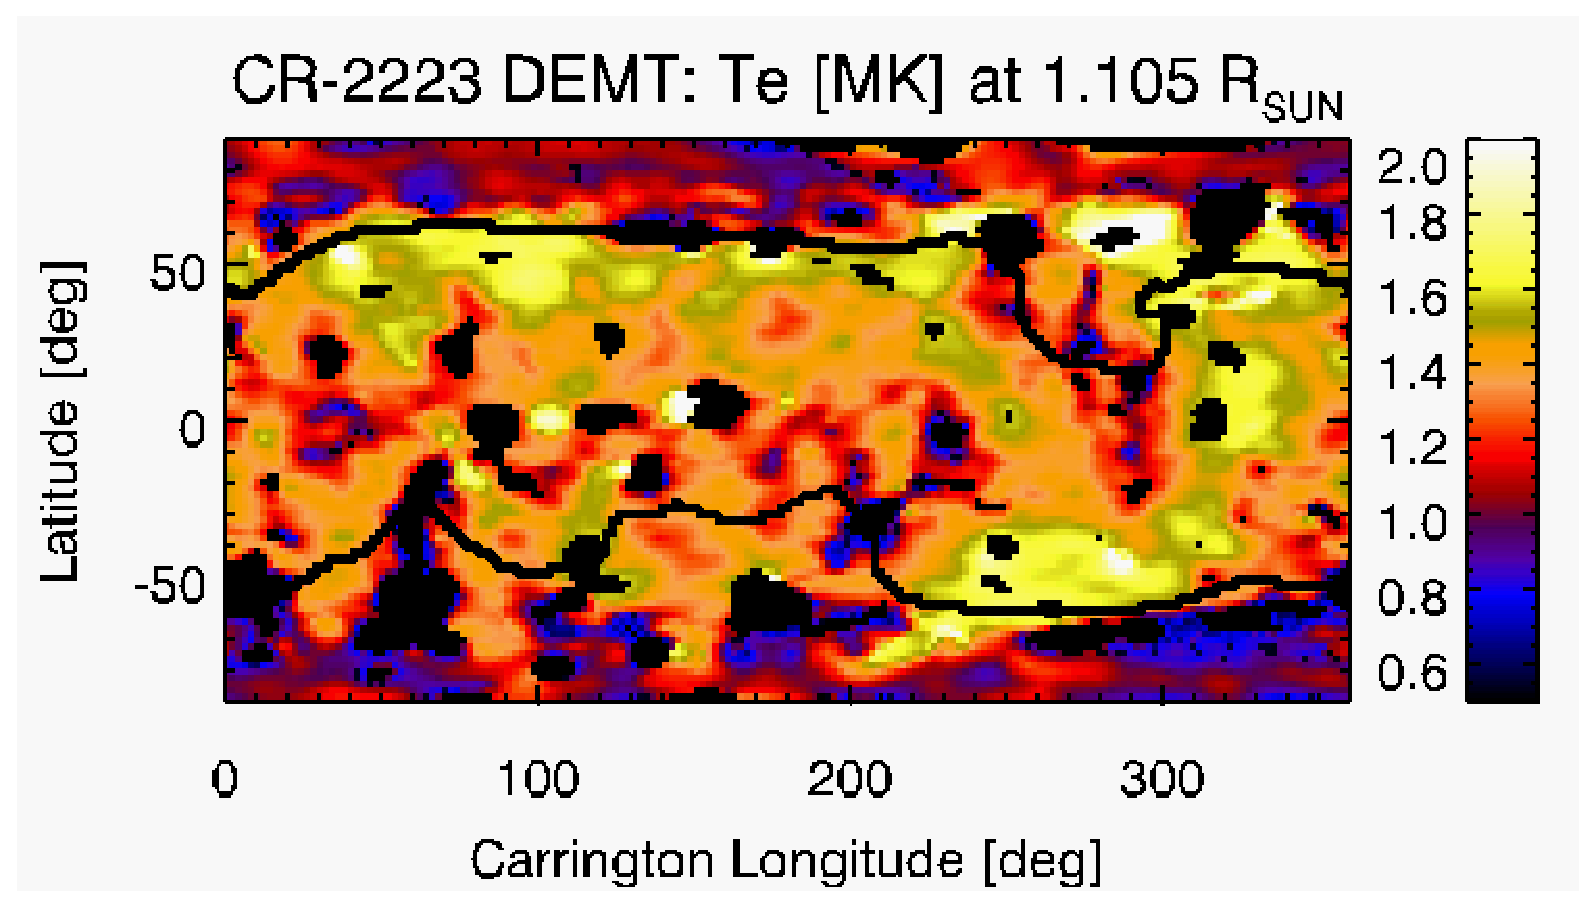
\includegraphics[width=0.95\textwidth,clip=]{figuras/map_Tm_CR2223_DEMT-AIA_H1_L733_r3d_multistart_1105_Rsun2223_2.eps}

\end{columns}  
Lloveras et al. (2017,2020,2022)\\
\vskip 0.3cm
\bu Azimuth symmetry\\
\bu Streamer(CHs) $\rightarrow$ higher(lower) density and temperature.\\
\bu Maximum gradients at O/C boundary\\
%\bu Simetría acimutal\\
%\bu Streamer(CHs) $\rightarrow$ mayor(menor) densidad y temperatura.\\
%\bu Gradientes máximos en frontera A/C
}
}


%------------------- PFSS
{
\setbeamercolor{title}{fg=blue}
\setbeamercolor{normal text}{fg=black}
\setbeamercolor{frametitle}{fg=blue}
\usebeamercolor[fg]{normal text}
\usebackgroundtemplate{{
\includegraphics[width=\paperwidth]
{figuras/fondo_poster_70x90cm.pdf}}}
\frame{
\titulo{3D magnetic model}
\begin{columns}

%\column{0.3\textwidth}
%\centering Magnetograma
%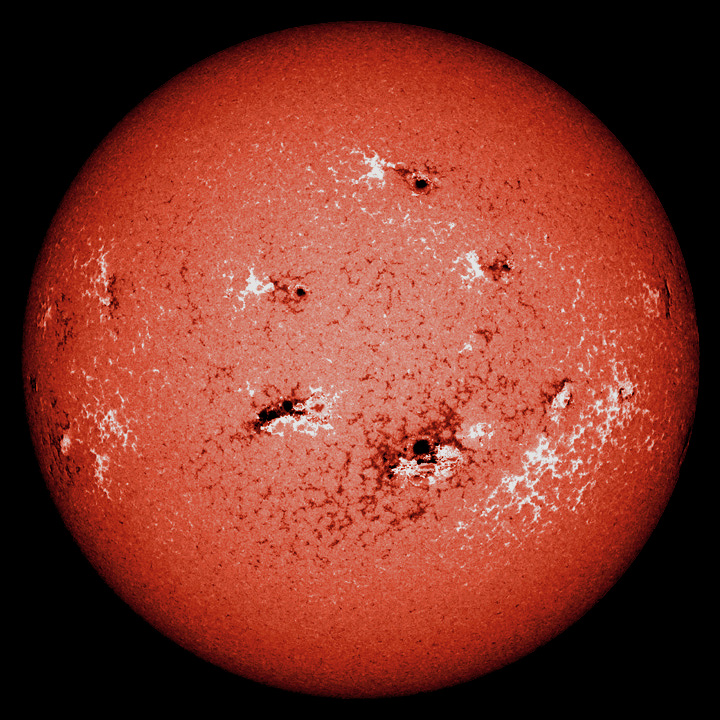
\includegraphics[width=0.99\textwidth]{figuras/magnetograma_esferico2.jpg}

%\column{0.3\textwidth}
%\centering Magnetograma sinóptico
%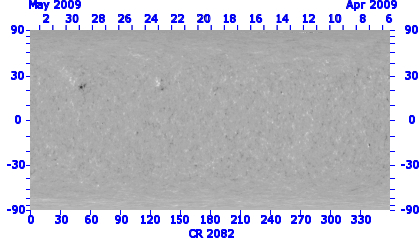
\includegraphics[width=0.99\textwidth]{figuras/mrmqj090419t1341c2082_000.jpg}

\column{0.5\textwidth}
\centering 
Sinoptic magnetogram ($\sim$ 28 days)\\
\includegraphics[width=0.99\textwidth]{figuras/fig1_nishtha2019_gong.pdf}\\
\includegraphics[width=0.99\textwidth]{figuras/fig1_nishtha2019_adapt_gong.pdf}

%\column{0.4\textwidth}
\column{0.5\textwidth}
\centering PFSS
\includegraphics[width=0.99\textwidth]{figuras/CR2081.jpg}
\end{columns}
\bu \small{Assimilation Photospheric Flux Transport (ADAPT, Worden and Harvey, 2000): applies a magnetic flux transport model.}
}
}


%-------------------------------TRAZADO
{
\setbeamercolor{title}{fg=blue}
\setbeamercolor{normal text}{fg=black}
\setbeamercolor{frametitle}{fg=blue}
\usebeamercolor[fg]{normal text}
\usebackgroundtemplate{{\includegraphics[width=\paperwidth]
{figuras/fondo_poster_70x90cm.pdf}}}
\frame{
\titulo{Tomographic Results along B-lines}
\footnotesize
%\begin{columns}
%\column{0.5\textwidth}
\includegraphics[height=0.35\linewidth]{figuras/Grid-loops.png}
%\includegraphics[height=0.35\linewidth]{figuras/Traced-Loop.eps}
\includegraphics[height=0.35\linewidth]{figuras/Traced-Loop_con_highpoints.pdf}
%\column{0.5\textwidth}
%\includegraphics[width=0.8\textwidth]{figuras/loop_Ne2.jpg}
%\includegraphics[width=0.8\textwidth]{figuras/loop_T2.jpg}
%\end{columns}
%\begin{center}
\salto
\begin{columns}
\column{0.6\textwidth}
%Results along individual {\bf B}-lines are characterized by parametric fits:
Results along individual B-lines are characterized by parametric fits:\\
%\begin{eqnarray*}
%\Ne(h) &=& N_0\ \textsf{exp}\left(-h/\lambda\right)
$ N_e^{\rm (EUV-SRT)} = N_0\, \exp{[-(h/\l)]}$\\
$ T_m = ar + b$\\
%\\
%\Te(h) &=& T_0 \, + \, \gamma \, h
%$$\hfill \ \ \ \ \ \ \ \ T_m = ar + b$$
%\end{eqnarray*}
%and fitting parameters are analyzed statistically.\\
and fitting parameters are analyzed statistically\\
\rojo{UP} \, \, \,  $(a \equiv \dTm_dr>0)$\\
\azul{DOWN} $(a \equiv \dTm_dr<0)$
\column{0.4\textwidth}
\includegraphics[width=0.99\textwidth]{figuras/table1_lloveras_2022.png}
%\centering
%\begin{tabular}{c c c }
%\hline
%  Type  & Characteristic     \\
%\hline
%   0   & \azul{Closed Small Down}   \\
%   I   & \orange{Closed Small Up}   \\
%   II  & \rojo{Closed Large Up}     \\
%   III & \cian{Open Large Up}    \\
%\hline
%\end{tabular}
%\includegraphics[width=0.99\textwidth]{figuras/tabla1_paper.png}
\end{columns}
%\end{center}
}
}

%------------------------------- Results
{
\setbeamercolor{title}{fg=blue}
\setbeamercolor{normal text}{fg=black}
\setbeamercolor{frametitle}{fg=blue}
\usebeamercolor[fg]{normal text}
\usebackgroundtemplate{{\includegraphics[width=\paperwidth]
{figuras/fondo_poster_70x90cm.pdf}}}
\frame{ 
\titulo{Results}
\footnotesize
\centering
\includegraphics[width=0.73\textwidth]{figuras/histograms_lloveras_2022.png}
}
}




{
\setbeamercolor{title}{fg=blue}
\setbeamercolor{normal text}{fg=black}
\setbeamercolor{frametitle}{fg=blue}
\usebeamercolor[fg]{normal text}
\usebackgroundtemplate{{\includegraphics[width=\paperwidth]
{figuras/fondo_poster_70x90cm.pdf}}}
\frame{ 
\titulo{Results DEMT}
\footnotesize
\begin{columns}
\column{0.5\textwidth}
\begin{center}
$N_e^{\rm (DEMT)}(r) = N_0\,\exp{\left[\,-\,\left(h/\l\right)\,/\,\left(r/{\rm R_\odot}\right)\,\right]}$\\
$T_e^{\rm (DEMT)}(r) = T_0\,+\,a\,h\ $ \\
$h \equiv r - 1\,\mrsun$ 
      

\end{center}


\column{0.5\textwidth}
\begin{center}
\includegraphics[width=0.9\textwidth]{figuras/table2_lloveras_2022.png}
lloveras et al. 2022
\end{center}

\end{columns}

}
}


%----------------------------

{
\setbeamercolor{title}{fg=blue}
\setbeamercolor{normal text}{fg=black}
\setbeamercolor{frametitle}{fg=blue}
\usebeamercolor[fg]{normal text}
\usebackgroundtemplate{{\includegraphics[width=\paperwidth]
{figuras/fondo_poster_70x90cm.pdf}}}
\frame{ 
\titulo{Results WL-SRT}
\footnotesize
\begin{columns}
\column{0.5\textwidth}
\begin{center}


$N_e^{\rm (C2-SRT)}(r) = N_0\,\left(\,r/2.5\,{\rm R_\odot}\right)^{-p} $

$ \langle \l \rangle \equiv  \left\langle \left|  \frac{1}{{\Ne(r)}} \, \frac{{{\rm d}\Ne}}{{\rm d}r}(r) \right|^{-1} \right\rangle {= \frac{\langle r\rangle}{p} = \frac{4.25\,\mrsun}{p}} $
\end{center}


\column{0.5\textwidth}
\begin{center}
\includegraphics[width=0.99\textwidth]{figuras/table3_lloveras_2022.png}
\end{center}

\end{columns}
}
}


%----------------------------


%---------------------- EUV-SRT vs AWSOM
{
\setbeamercolor{title}{fg=blue}
\setbeamercolor{normal text}{fg=black}
\setbeamercolor{frametitle}{fg=blue}
\usebeamercolor[fg]{normal text}
\usebackgroundtemplate{{\includegraphics[width=\paperwidth]
{figuras/fondo_poster_70x90cm.pdf}}}
\frame{ 
\titulo{EUV-SRT validation of AWSoM}
\scriptsize
%\bu Objetivo: Validar la capacidad del modelo en reproducir las reconstrucciones.
%\bu Motivación: Es AWSoM capaz para reproducir las reconstrucciones tomográficas?
\vskip -0.2cm
\begin{columns}
\column{0.7\textwidth}
\begin{center}
\includegraphics[width=0.49\textwidth]{figuras/map_Ne_CR2223_DEMT-AIA_H1_L733_r3d_multistart_1105_Rsun2223.eps}
\includegraphics[width=0.49\textwidth]{figuras/map_Tm_CR2223_DEMT-AIA_H1_L733_r3d_multistart_1105_Rsun2223_2.eps}\\
\includegraphics[width=0.49\textwidth]{figuras/map_Ne_awsom_2223_ener_new_1105_Rsun2223.eps}
\includegraphics[width=0.49\textwidth]{figuras/map_Te_awsom_2223_ener_new_1105_Rsun2223_2.eps}\\
\includegraphics[width=0.49\textwidth]{figuras/perfil_paper_necr2223_bajo.eps}
\includegraphics[width=0.49\textwidth]{figuras/perfil_paper_tecr2223_bajo.eps}\\
\end{center}
\column{0.3\textwidth}
\bu Good agreement in magnitude and morphology of structures.\\
\vskip 0.4cm
\bu Good agreement North O/C boundary and CH\\
\vskip 0.4cm
\bu Southern O/C boundary shifted $+20\mdeg$ from CH\\
\vskip 0.4cm
\bu $\Delta T_e(r) \sim -15\%$ \\
\vskip 0.4cm
\bu $\Delta N_e(r) \sim 5\%$\\
\vskip 2cm
\hfill (Lloveras et al. 2022)
\end{columns}
}
}
%--------------- imág sintéticas
{
\setbeamercolor{title}{fg=blue}
\setbeamercolor{normal text}{fg=black}
\setbeamercolor{frametitle}{fg=blue}
\usebeamercolor[fg]{normal text}
\usebackgroundtemplate{{\includegraphics[width=\paperwidth]
{figuras/fondo_poster_70x90cm.pdf}}}
\frame{
\titulo{EUV Synthetic Images: EUV-SRT vs AWSoM}
\vskip -3cm
\begin{center}
\includegraphics[width=0.99\textwidth,clip=]{figuras/Figura_2_paper_imag_sinteticas_2.eps}
\end{center}

\begin{columns}
\column{0.35\textwidth}
$I_{Synt} \sim \int_{LoS} \mathrm{d}l \, N_e^2 \, Q_k$\\
%\vskip 0.2cm


\column{0.65\textwidth}
%\scriptsize
\bu  AWSoM O/C discrepancy due to lack of accuracy of boundary condition.\\ 
\hfill (Lloveras et al. 2022)\\
\end{columns}
%\bu AWSoM reproduce las Ne basales EUV-SRT con un acuerdo $\simeq$ 10\% \\
%\bu La $\lambda_N$ y temperatura simuladas son sistemáticamente 5-20\% menores.
}
}




%-----------------------------------------

















\end{document}

% Slides extra
